%==============================================================
%  APIGUARD -- Deliverable 2: System Model and Description
%  CSS453 Term Project, SIIT, Thammasat University
%  IEEE conference format (IEEEtran).
%  Compile on Overleaf with pdfLaTeX. No bibtex pass is needed:
%  the bibliography is written out with thebibliography below.
%  A refs.bib is included if you prefer \bibliography{refs}.
%==============================================================
\documentclass[conference]{IEEEtran}
\IEEEoverridecommandlockouts

\usepackage{cite}
\usepackage{amsmath,amssymb}
\usepackage{graphicx}
\usepackage{array}
\usepackage{tabularx}
\usepackage{booktabs}
\usepackage{listings}
\usepackage{algorithm}
\usepackage{algorithmic}
\usepackage{xcolor}
\usepackage{url}
\usepackage[hidelinks]{hyperref}

\newcolumntype{L}[1]{>{\raggedright\arraybackslash}p{#1}}
\newcolumntype{Y}{>{\raggedright\arraybackslash}X}

\lstset{
  basicstyle=\ttfamily\scriptsize,
  breaklines=true,
  frame=single,
  framesep=3pt,
  columns=fullflexible,
  keepspaces=true,
  showstringspaces=false,
  xleftmargin=2pt,
  aboveskip=6pt,
  belowskip=4pt
}

\begin{document}

\title{APIGUARD: A Machine Learning-Assisted Framework for\\
Continuous API Security Assessment in DevSecOps Pipelines\\
\large Final Report --- System Model, Methodology and Results}

\author{\IEEEauthorblockN{Thornkasidej Fuangfoo (6622771234) \quad Varit Mesri (6622771317)}
\IEEEauthorblockA{Sirindhorn International Institute of Technology (SIIT),
Thammasat University, Pathum Thani, Thailand\\
Adviser: Somchart Fugkeaw}
\thanks{This report describes the system for the registered topic
``Continuous API Security Assessment in DevSecOps Pipelines.'' It replaces the
Infrastructure-as-Code system presented in Deliverable~1, which was withdrawn because that
topic had already been reserved by another group. The target artefact is now the OpenAPI specification instead of Terraform code.}}

\maketitle

\begin{abstract}
Rule-based linting is the only security check most OpenAPI specifications receive before
deployment. A linter fires when a written rule matches, which leaves it unable to say which
findings matter, unable to distinguish an endpoint returning a health-check string from one
returning customer records, and silent about anything no rule covers. In a CI/CD pipeline
this produces alert fatigue and blind spots at the same time. This paper presents
APIGUARD, a framework that places a supervised classifier \emph{after} the
rule scanner rather than in place of it. The scanner keeps its authority over what rules
cover; the model assigns every endpoint a risk score, ranks the findings, and explains each
score with SHAP attributions, so that the pipeline gate acts on a risk score rather than on
an alert count. We define the entities and their trust relationships, the notation and the
gate decision rule, every runtime and offline component with its inputs, outputs and
guarantees, the data flow of a single pipeline run, the threat model and its stated limits,
and the deployment form. We also map each research question to the experiment that
answers it. The methodology section then specifies how labels are made and kept apart from the
scanner's own output, the training algorithm, a gate that judges only new or changed endpoints,
and the rule hold-out protocol that tests whether the model generalises beyond the rules.
Trained on scanner labels the model matches but does not beat the scanner (PR-AUC 0.42 against 0.47); trained on language-model reference labels it ranks better by ROC-AUC (0.84 against 0.69), and combined with the scanner it ranks better on both PR-AUC (0.55 against 0.47) and ROC-AUC. The rule hold-out generalises for one of three testable categories, and the model ranks the documented flaws of VAmPI but not those of crAPI. After adviser feedback the corpus was extended with 368 specifications from 25 further sources, OWASP ZAP was run against VAmPI and Damn Vulnerable RESTaurant as a real dynamic baseline (at medium risk or higher it flags one documented flaw endpoint in each application), and the feedback lane became an LLM checker followed by a random human audit (a person agreed with the checker on 28 of 28 audited verdicts). A revised model (v3) that keeps each scanner finding with its own endpoint, drops the context features and adds fourteen flaw-pattern features reaches PR-AUC 0.62 and ROC-AUC 0.85 against 0.47 and 0.69 for the scanner, with both provider-level intervals excluding zero; it still does not rank the flaws of crAPI, because the reference labels rarely mark an authenticated endpoint as risky.
\end{abstract}

\begin{IEEEkeywords}
API security, OpenAPI, DevSecOps, CI/CD, static analysis, XGBoost, SHAP, OWASP API Security
Top 10, risk scoring.
\end{IEEEkeywords}

%==============================================================
\section{Introduction}
Modern software is assembled out of HTTP APIs, and the OpenAPI specification is the first
place where an API's security posture is written down: which endpoints require
authentication, which scheme they use, what data comes back, and what limits apply. That
makes the specification a cheap and early place to catch security design mistakes, long
before a penetration test is run.

Today this checking is done by rules only. A linter such as Spectral with the OWASP ruleset
fires when a written rule matches. It cannot say which of its findings actually matter, it
produces the same alert whether an endpoint returns a health-check string or a customer's
date of birth, and it says nothing about a problem nobody wrote a rule for. Inside a CI/CD
pipeline this causes two failures at once: developers stop reading the alerts, and the gate
lets dangerous designs through.

Scale makes the opportunity concrete. The APIstic dataset contains 1{,}275{,}568 valid
OpenAPI specifications mined from GitHub, SwaggerHub, BigQuery and APIs.guru~\cite{apistic},
and the curated APIs.guru directory alone holds 2{,}529 API descriptions covering 108{,}837
endpoints~\cite{apisguru}. This is a large, machine-readable body of real-world API design,
and it is almost untouched as training data for security.

APIGUARD places a supervised model \emph{after} the rule scanner. The scanner keeps finding
what rules find; the model gives every endpoint a risk score, ranks the findings, and
explains each score with SHAP. The pipeline gate then acts on a risk score instead of a raw
alert count. This paper specifies the system model: the entities involved, the notation
used, every component with its inputs and outputs, the data flow of a single pipeline run,
the trust assumptions, and the way the system is deployed. It then specifies the proposed
methodology and algorithms (Section~\ref{sec:method}) and reports the experiments (Section~\ref{sec:results}).

The contributions are:
\begin{itemize}
\item A system model in which a classifier scores \emph{every} endpoint after the rule scanner,
so that the gate acts on a ranked, explained risk score instead of an alert count.
\item A label protocol that keeps scanner labels for training only and measures every reported
result against independently produced labels (L2 and L3), which removes from the evaluation the circularity of testing on
scanner output.
\item A rule hold-out protocol (E2) that tests whether the model learned a design property
rather than a rule trigger.
\item A gate that judges only new or changed endpoints, so that existing APIs can adopt it.
\item A working implementation of the normaliser (S0), the feature builder (S2a, 66 features)
and the gate (S3), each with contract tests.
\end{itemize}

\textbf{Changes since Deliverable 2.} The system model of Deliverable~2 is kept and revised
as follows: (i)~a fabricated author name was removed from the VAmPI reference; (ii)~the SHAP
contract now states that attributions sum to the raw margin, not to the score; (iii)~the claim
that a developer cannot change the threshold now names the mechanism that enforces it;
(iv)~the evaluation no longer scores the model against the scanner labels it trained on;
(v)~a text-inflation test was added; (vi)~the feature table now
matches the implemented feature builder; (vii)~the gate counts only new or changed
endpoints; and (viii)~the feedback lane is an LLM checker followed by a random human audit of its verdicts (Section~\ref{sec:feedback}); (ix)~the corpus was extended with specifications from 25 further sources (Section~\ref{sec:corpus-ext}); and (x)~OWASP ZAP~\cite{zap}, a real OWASP dynamic scanner, was run against VAmPI and compared with APIGUARD (Section~\ref{sec:e10}).

%==============================================================
\section{Related Work}
\subsection{Analysis of OpenAPI Specifications}
Serbout and Pautasso collected 1{,}275{,}568 OpenAPI specifications and published structural
metrics for them~\cite{apistic}; their work describes how APIs are written, not how safe the
designs are. Decrop \emph{et al.} automate the quality analysis of OpenAPI
specifications~\cite{oasquali}. The closest work to ours, Cheh and Chen, analyse OpenAPI
documents for security design issues with a graph model of sensitive-field exposure, but
evaluate it on a single API~\cite{cheh}. Tanveer \emph{et al.} survey the detection of
vulnerabilities in RESTful APIs~\cite{tanveer}.

\subsection{Rule-Based Scanning and Alert Prioritisation}
Spectral with the OWASP ruleset turns the API Security Top 10 into rules that fire on a
specification~\cite{spectralowasp,owasptop10}. A rule fires or it does not; it gives no ranking
and cannot report a problem nobody wrote a rule for. Flynn \emph{et al.} show that
classification models can prioritise the alerts of several static analysis tools~\cite{flynn}.
APIGUARD applies this idea at endpoint level to API specifications, and additionally scores
endpoints on which no rule fired.

\subsection{Weak Labels and Explanation}
Training on automatically produced labels falls in the weak-supervision setting described
for Snorkel~\cite{snorkel}. We do not fit Snorkel's label model; scanner output is used
directly as noisy labels, and because such labels are noisy, we use them for training only.
Gradient-boosted trees~\cite{xgboost} are explained with SHAP~\cite{shap} and its exact
tree algorithm~\cite{treeshap}. Leakage between training and test data is a documented cause of
over-optimistic results~\cite{kapoor}, which is why every split here is grouped by provider.

\subsection{Gap}
To our knowledge, no existing work combines a learned, explained, endpoint-level risk score
with a pipeline gate and tests it on rules that were held out of training. This is the gap
APIGUARD addresses.

%==============================================================
\section{System Overview}
APIGUARD is organised into three lanes. Separating them is a design decision rather than a
drawing convenience: each lane runs at a different time, under different trust conditions,
and at a different speed.

\begin{itemize}
\item The \textbf{runtime lane} is what ships. It runs on every commit inside the CI/CD
pipeline, must finish in seconds, and is fully automatic.
\item The \textbf{offline lane} builds the model. It runs rarely, on a workstation or build
server, and may take hours.
\item The \textbf{feedback lane} is how a corrected verdict re-enters the system. It is
an LLM checker labels the uncertain endpoints and a person checks a random sample of its verdicts; it is deliberately slow and never reaches the model directly.
\end{itemize}

Fig.~\ref{fig:arch} shows the three lanes and the two connections between them: the trained
model artefact loaded by the runtime, and the shared code path that guarantees training and
runtime compute features identically.

\begin{figure*}[!t]
\centering
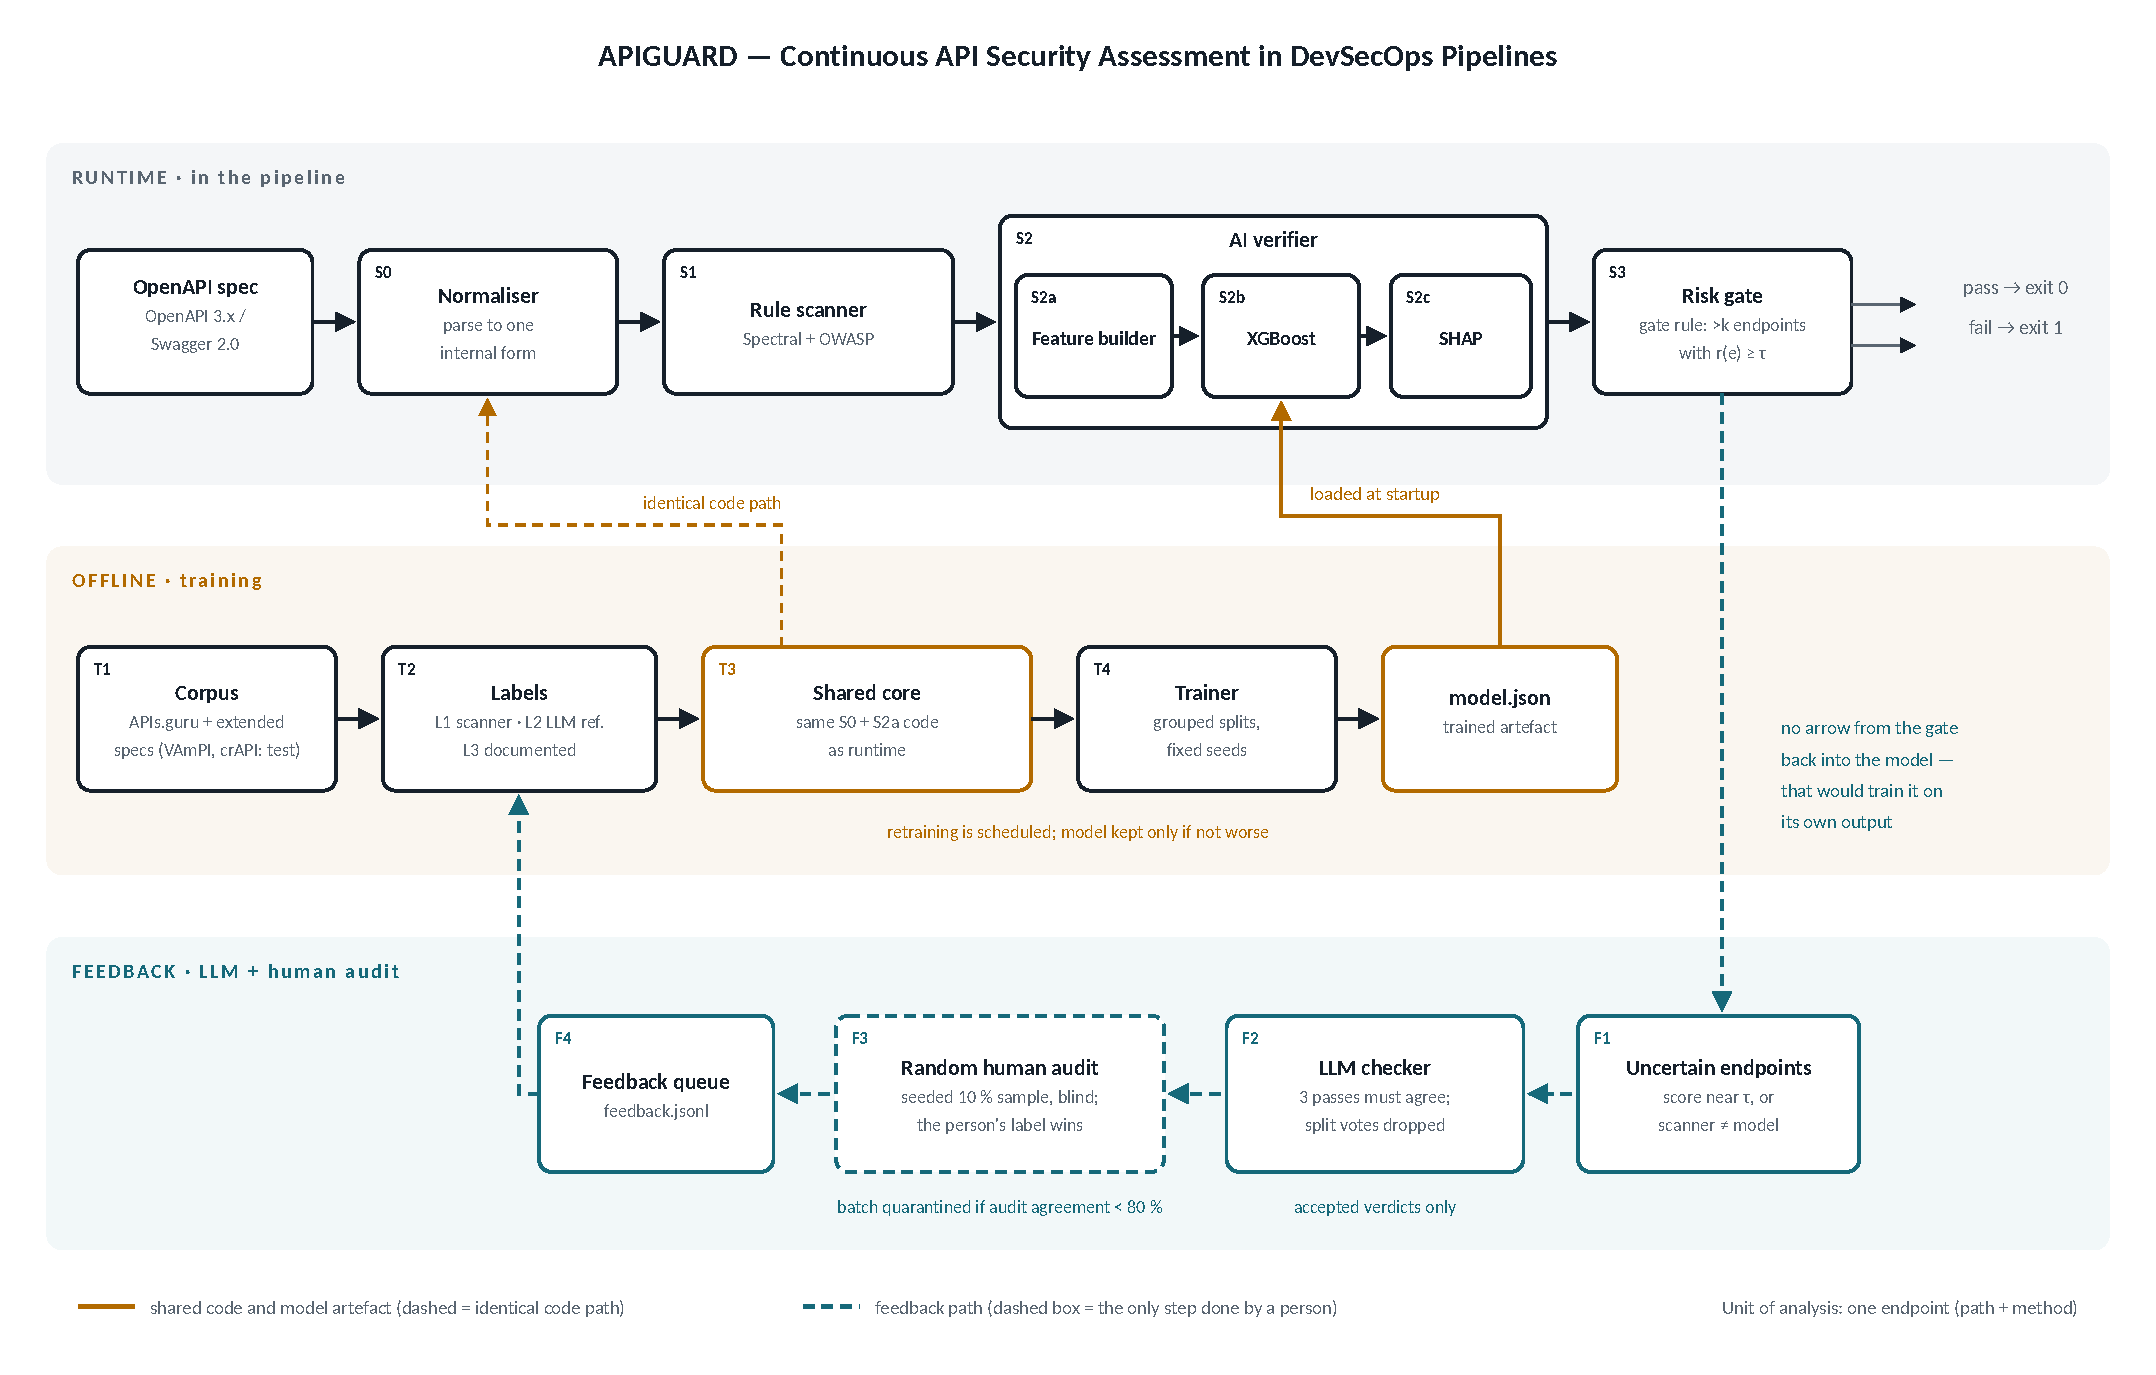
\includegraphics[width=\textwidth]{architecture_v4.pdf}
\caption{APIGUARD system model. The runtime lane (S0--S3) runs inside the pipeline; the
offline lane (T1--T4) produces \texttt{model.json}; the feedback lane returns LLM-checked verdicts, audited at random by a person,
to the label store. Amber marks shared code and the model artefact; dashed teal marks
the feedback path, and its dashed box is the one step done by a person. The unit of analysis is one endpoint.}
\label{fig:arch}
\end{figure*}

%==============================================================
\section{Entities, Roles and Trust Assumptions}
Six entities take part in the system. Table~\ref{tab:entities} states the role of each and
how far it is trusted.

\begin{table*}[!t]
\caption{Entities, Their Roles and Trust Assumptions}
\label{tab:entities}
\centering
\footnotesize
\begin{tabularx}{\textwidth}{L{2.4cm} Y Y}
\toprule
\textbf{Entity} & \textbf{Role in the system} & \textbf{Trust assumption}\\
\midrule
Developer & Writes or edits an OpenAPI specification and pushes it to the repository; reads
the gate output and fixes what it reports. & Not malicious, but assumed to make design
mistakes. Cannot change the gate threshold, the tolerance or the model artefact used on a
protected branch: the gate runs from an organisation-level required workflow or a repository
ruleset rather than from a workflow file in the pull request, the workflow files and the
\texttt{models/} directory are covered by CODEOWNERS, and the required workflow checks the
SHA-256 hash of \texttt{model.json} against a value pinned outside the repository. Branch
protection alone is not sufficient, because it blocks merging but not running a modified
workflow.\\
CI/CD runner & Checks out the repository, invokes the APIGUARD CLI, and acts on its exit
code. & Trusted execution environment; its configuration is under version control.\\
APIGUARD CLI & The runtime lane, S0--S3. Reads a specification and produces a per-endpoint
risk report and a pass/fail exit code. & The component under study. Must be deterministic
for a fixed specification, ruleset version and model.\\
Rule scanner & Third-party linter (Spectral with the OWASP ruleset). Supplies findings used
as a baseline and as model input. & Trusted but incomplete. Version is pinned, because a
version change silently changes every label.\\
LLM checker and human auditor (replace the human analyst of Deliverable~2) & The checker re-labels the endpoints whose verdict is in doubt with three independent language-model passes and keeps a label only when all three agree. A person labels a seeded random sample of the accepted verdicts without seeing them. & The checker is trusted only when unanimous. The person's label always wins on the audited rows, and a batch whose audit agreement is below 80\,\% is quarantined (Section~\ref{sec:feedback}).\\
Offline trainer & Builds the corpus, assembles labels, trains the model and emits
\texttt{model.json}. & Runs outside the pipeline. Never invoked automatically by a gate
decision.\\
\bottomrule
\end{tabularx}
\end{table*}

%==============================================================
\section{Notation and Definitions}
Table~\ref{tab:notation} fixes the notation used here and in every later deliverable.

\begin{table*}[!t]
\caption{Notation Used Throughout the Project}
\label{tab:notation}
\centering
\footnotesize
\begin{tabularx}{\textwidth}{L{2.6cm} Y}
\toprule
\textbf{Symbol} & \textbf{Meaning}\\
\midrule
$S$ & An OpenAPI 3.x or Swagger 2.0 specification document; the input to one pipeline run.\\
$e=(p,m)$ & One \emph{endpoint}: a path $p$ combined with an HTTP method $m$. This is the
unit of analysis.\\
$E(S)$ & The set of all endpoints declared in $S$, produced by the normaliser S0.\\
$A(e)$ & The scanner findings attributed to $e$, each carrying a rule identifier, a severity
and an OWASP API Top 10 category.\\
$x(e)\in\mathbb{R}^{d}$ & The feature vector of $e$, produced by S2a from the normalised
specification and from $A(e)$.\\
$y(e)\in\{0,1\}$ & The label of $e$: 1 if the endpoint carries a security-relevant design
issue, 0 otherwise.\\
$f:\mathbb{R}^{d}\!\rightarrow\![0,1]$ & The trained classifier (XGBoost), loaded from
\texttt{model.json} at CLI startup.\\
$r(e)$ & The risk score of $e$, defined as $r(e)=f(x(e))$.\\
$\phi(e)$ & The SHAP attribution vector for $e$: the contribution of each feature to the raw margin
(log-odds) from which $r(e)$ is computed.\\
$\tau,\;k$ & The gate threshold and the tolerated count of endpoints at or above it.\\
$G(S)$ & The gate decision for the whole specification: $0$ = pass, $1$ = fail.\\
$\mathrm{P@}n$ & Precision among the $n$ highest-ranked findings (Experiment~E3). Written with
$n$ so that it is not confused with the gate tolerance $k$.\\
\bottomrule
\end{tabularx}
\end{table*}

For one specification $S$, the runtime lane computes the scored endpoint set
\begin{equation}
R(S)=\bigl\{\,\bigl(e,\;r(e),\;\phi(e)\bigr)\;:\;e\in E(S)\,\bigr\},
\label{eq:scored}
\end{equation}
and the gate decision is
\begin{equation}
G(S)=
\begin{cases}
1, & \bigl|\{\,e\in E(S)\;:\;r(e)\ge\tau\,\}\bigr| > k,\\[2pt]
0, & \text{otherwise.}
\end{cases}
\label{eq:gate}
\end{equation}

Equation~\eqref{eq:gate} is the full-scan form of the gate. The deployed gate, defined
in~\eqref{eq:gatedelta} of Section~\ref{sec:m-gate}, applies the same rule only to endpoints
that are new or changed relative to the base branch; \eqref{eq:gate} is the special case in
which no base specification exists, so that every endpoint counts as new.

With the default policy $k=0$ the gate fails if any single endpoint scores at or above
$\tau$. A larger $k$ lets a team adopt the tool gradually on an existing API without
blocking every build on the first day. The value of $\tau$ is not chosen by hand: it is
selected on validation folds (Section~\ref{sec:m-gate}), stored in the metadata of
\texttt{model.json}, and its precision/recall trade-off is reported in Experiment~E3.

Two properties the design must hold. First, $r(e)$ is defined for \emph{every} endpoint,
including endpoints on which no rule fired; for those, the scanner-derived features are
simply zero. Second, for a fixed specification, ruleset version and model artefact the whole
runtime lane is deterministic --- nothing in it samples randomly.

%==============================================================
\section{Runtime Lane: Components S0--S3}

\subsection{S0 --- Normaliser}
\textbf{Input:} a specification file in YAML or JSON, either OpenAPI 3.x or Swagger 2.0.
\textbf{Output:} a list of normalised endpoint records, one per (path, method) pair.

The normaliser resolves internal \texttt{\$ref} pointers, expands the schema of every request
body and response, and flattens the two specification versions into one internal form, so
that the rest of the pipeline reads one record format. The version is kept only as the feature \texttt{is\_oas3} and for per-version reporting. Path-level
parameters are merged into each operation, and a global \texttt{security} block is propagated
to operations that do not declare their own --- recording, importantly, whether the operation
\emph{inherited} or \emph{overrode} that requirement. An operation that explicitly overrides
global security with an empty requirement is a different risk from one that simply inherits
it, and a design that collapsed the two would lose that distinction before the model ever
saw it.

\textbf{Guarantees.} Every endpoint of a parsable specification appears exactly once in the
output. A specification that cannot be parsed is not silently skipped: it is written to an
error log with the reason, and the corpus statistics report the parse-failure rate. Circular
references are cut at a fixed depth so that expansion always terminates.

\subsection{S1 --- Rule Scanner}
\textbf{Input:} the original specification file. \textbf{Output:} the set $A(e)$ of findings
for each endpoint.

S1 runs Spectral with \texttt{@stoplight/\allowbreak spectral-\allowbreak owasp-\allowbreak ruleset}~v2.x, which implements the
OWASP API Security Top 10, 2023 edition~\cite{owasptop10,spectralowasp}. Spectral reports
findings against JSON paths inside the document; S1 maps each finding down to the endpoint it
belongs to, so that a document-level finding is attributed to every endpoint and an
operation-level finding only to its own. The 42Crunch audit score was not collected.

S1 output is used in three distinct ways, and keeping them apart matters for the evaluation:
it is the \textbf{baseline} the model is compared against, it is the source of the
\textbf{automatic labels} used for training, and it enters the model as \textbf{input
features}. The scanner and ruleset versions are pinned and recorded in every report, because
a ruleset upgrade changes both the baseline and the labels at the same time.

\subsection{S2 --- AI Verifier}
S2 is the core of the contribution and has three sub-components.

\textbf{S2a Feature builder.} Turns one normalised endpoint record, plus its scanner
findings, into a fixed-length numeric vector $x(e)$. The features fall into the six groups of
Table~\ref{tab:features}. The builder is a tested module with no dependency on the training
pipeline, which is what allows the same code to be imported by both S2a and T3.

\textbf{S2b Classifier.} An XGBoost gradient-boosted tree ensemble~\cite{xgboost}, loaded
from \texttt{model.json} at startup and applied to every endpoint. Gradient boosting is
chosen because the input is a table of mixed numeric, binary and categorical features,
because strong class imbalance is handled directly through \texttt{scale\_pos\_weight}, and
because tree ensembles remain traceable back to individual features. Simpler baselines ---
majority class, logistic regression and random forest --- are trained on the identical
feature table for comparison.

\textbf{S2c Explainer.} SHAP~\cite{shap} produces $\phi(e)$, attributing the score to
individual features using Shapley values from cooperative game theory, computed exactly for
tree ensembles by TreeSHAP~\cite{treeshap}. Every endpoint that counts toward the gate
decision, and each of the ten highest-scoring endpoints, carries up to three features
that pushed its score up (Algorithm~\ref{alg:scan}). This is not decoration: it is how a
developer checks whether the model reasoned about a security property or about something
irrelevant, and it is how the team detects a model that has learned a shortcut.

\begin{table*}[!t]
\caption{Feature Groups Computed by S2a From One Normalised Endpoint}
\label{tab:features}
\centering
\footnotesize
\begin{tabularx}{\textwidth}{L{2.2cm} Y L{4.6cm}}
\toprule
\textbf{Group} & \textbf{Contents} & \textbf{Why it should carry signal}\\
\midrule
A. Structural & Path depth; number of path parameters; whether a path parameter looks like an
object identifier (\texttt{id}, \texttt{uuid}, \texttt{\_id}); HTTP method; query and header
parameter counts; request body present; response schema property count; declared status
codes; whether 401/403 are declared; deprecated flag. & An object identifier in the path with
no ownership check is the classic API1 Broken Object Level Authorization shape.\\
B. Security scheme & Whether the endpoint has a security requirement; inherited versus
overridden; scheme type (apiKey, http-basic, http-bearer, oauth2, openIdConnect); scope
count; whether the server URL uses \texttt{http} rather than \texttt{https}. & The direct
expression of authentication and authorisation design (API2, API5).\\
C. Data sensitivity & Count of response property names matching a sensitive-term lexicon
(password, token, secret, ssn, dob, phone, email, address, card, balance); maximum term
weight; sensitive properties in response versus request; ratio of sensitive to total
properties; the combination flag \emph{no security requirement and sensitive response
fields}. & What a rule cannot see: it separates a health-check endpoint from one returning
customer data (API3).\\
D. Documentation hygiene & Description and summary lengths; example present; share of
parameters with a description or example; version segment in the path; pagination parameters present; rate-limit headers
documented. & Poorly specified endpoints correlate with weak design; rate-limit documentation
relates to API4.\\
E. Scanner-derived & \texttt{flagged\_by\_spectral}, \texttt{rule\_count},
\texttt{severity\_max}, the number of OWASP categories hit and one flag per category. All zero when nothing fired. & Lets the model use the rules' output as evidence. The model may come to copy this group; it is kept separable so the ablation (E5) and the rule hold-out (E2) can test for that.\\
F. Context & Endpoint count of the parent specification; whether the file is OpenAPI 3.x
or Swagger 2.0. Provider identity is deliberately excluded and used only to group the splits. & Places the endpoint inside its API rather than judging it in
isolation.\\
\bottomrule
\end{tabularx}
\end{table*}

\subsection{S3 --- Risk Gate}
\textbf{Input:} $R(S)$, the scored endpoint set. \textbf{Output:} a report and a process exit
code.

S3 applies the decision rule of~\eqref{eq:gatedelta}, which reduces to~\eqref{eq:gate} when no
base specification is given, and emits the ranked findings in one of three formats:
human-readable text for a terminal, JSON for further processing, and SARIF so that results
appear as annotations in the code-review interface. The exit code is 0 on pass and 1 on fail,
which is the only part of the system the CI runner needs to understand. The report always
lists endpoints in descending risk order. Each entry carries the score and any scanner
findings that fired; entries that count toward the gate decision or are among the ten highest
scores also carry their SHAP reasons.

%==============================================================
\section{Offline Lane: Components T1--T4}

\subsection{T1 --- Corpus}
Table~\ref{tab:corpora} lists the sources; APIs.guru, the added sources of Section~\ref{sec:corpus-ext}, VAmPI and crAPI were used. Each downloaded specification is stored with
its source URL and a snapshot date, and is de-duplicated by a hash of the file text before
anything else happens. Public API specifications are heavily copied and templated between
projects; near-duplicates left in the corpus would appear on both sides of a train/test
split.

\begin{table}[!t]
\caption{Corpora and Their Role in the Project}
\label{tab:corpora}
\centering
\footnotesize
\begin{tabularx}{\columnwidth}{L{1.7cm} L{1.9cm} Y}
\toprule
\textbf{Source} & \textbf{Size} & \textbf{Use}\\
\midrule
APIs.guru~\cite{apisguru} & 2{,}529 APIs, 108{,}837 endpoints & Primary corpus; curated,
clean, version-stable.\\
Added sources (Sec.~\ref{sec:corpus-ext}) & 368 specifications, 9{,}741 endpoints, 25 GitHub owners & Variety: telecom, banking, DevOps tools, IoT, generator test suites, vulnerable-by-design apps. Used for the transfer test E12, not for training.\\
APIstic~\cite{apistic} & 1{,}275{,}568 specifications & Not used for training; cited as related work and as a scale reference.\\
VAmPI~\cite{vampi} & 1 API, documented flaws & Ground truth: flaws documented by the
authors, mapped to endpoints.\\
OWASP crAPI~\cite{crapi} & 1 API, documented challenges & Second ground-truth target,
independent of VAmPI.\\
\bottomrule
\end{tabularx}
\end{table}

\subsection{T2 --- Label Store}
Three label sources are kept separate and never merged into one undifferentiated pile.

\begin{itemize}
\item \textbf{L1 automatic.} Spectral OWASP findings mapped down to endpoints. Cheap and
plentiful, and circular if used alone --- a model trained only on L1 can at best reproduce
the scanner.
\item \textbf{L2 reference labels.} A stratified sample of 304 endpoints labelled independently
by three language-model passes that never saw scanner output or model scores, combined by
majority vote, with agreement reported as Cohen's~\cite{cohen} and Fleiss'~\cite{fleiss} $\kappa$. No human labelled
these endpoints; a random sample of 23 plus 5 extra rows (28 in all) was audited by a person (Section~\ref{sec:e11}). Small and imperfect, but independent of the scanner, which is what the
false-positive claim needs.
\item \textbf{L3 ground truth.} VAmPI and crAPI endpoints with known, documented
vulnerabilities.
\end{itemize}

\subsection{T3 --- Shared Core}
T3 is not a separate implementation. It is the S0 normaliser and the S2a feature builder
\emph{imported} by the training pipeline, not copied into it. This is a deliberate
constraint: if training and runtime computed features from two code paths, any drift between
them would appear as an unexplained drop in live accuracy that no experiment could diagnose.
The amber path in Fig.~\ref{fig:arch} marks this shared code.

\subsection{T4 --- Trainer}
T4 takes the labelled feature table and produces \texttt{model.json}. Four rules govern it.

\begin{enumerate}
\item \textbf{Split by provider or repository, never at random.} A random split leaks
near-identical endpoints across the boundary and produces impressive but meaningless scores.
Grouped 5-fold cross-validation is used throughout.
\item \textbf{Report PR-AUC, F1 and MCC, not accuracy.} Insecure endpoints are a small
minority; a model that predicted ``secure'' for everything would score high on accuracy
alone.
\item \textbf{Fix every random seed and record every dependency version.} The scanner version,
ruleset version, corpus statistics, seed and the selected threshold $\tau$ are written
into the model artefact's metadata; the snapshot date is kept in the corpus manifest.
\item \textbf{Emit an artefact, not a live service.} \texttt{model.json} is a file under
version control, so any reported result can be reproduced with the exact model that produced
it.
\end{enumerate}

%==============================================================
\section{Feedback Lane}
\label{sec:feedback}
After adviser feedback the lane has two checks in series: a language model checks the verdicts that are in doubt, and a person
then checks a random sample of the language model's work. The person is not a reviewer of every verdict (that does not scale
and was the weakness of Deliverable~2); the person is a quality control on the checker.

\textbf{Selection.} After a pipeline run, the endpoints whose verdict is in doubt are
selected: those whose score $r(e)$ lies within 0.10 of $\tau$, and those on which the model and the
scanner disagree (flagged by S1 but scored low, or not flagged but scored high).

\textbf{LLM checker.} Each selected endpoint is labelled by three independent
language-model passes that follow the codebook of Section~\ref{sec:method} and see neither
the scanner output nor the model score. A label is accepted only when all three passes agree;
split votes are discarded. Where the API can be run in a test environment, a failure that a
dynamic tester finds on an endpoint is also accepted as a positive label. A clean dynamic run
is not evidence of safety and is never accepted as a negative label.

\textbf{Random human audit.} A seeded random sample of the \emph{accepted} verdicts, 10\,\% and at least 20, is drawn
stratified by checker label (so the rare positives are not lost) and ordered by a hash of the seed and the endpoint identity, so that
the draw is reproducible and independent of the score. The person sees the same card the checker saw, with no checker verdict and no score,
and answers yes or no. On every audited row the person's label replaces the checker's. The batch is accepted when person and checker agree
on at least 80\,\% of the sample; otherwise the whole batch is quarantined and only the person-verified rows are kept. Agreement,
Cohen's~$\kappa$ and a Wilson~\cite{wilson} 95\,\% interval are reported for every batch. The 80\,\% rule and the 10\,\% rate are design choices, not tuned values.
Accepted records are appended to \texttt{feedback.jsonl}: the endpoint identity, the specification hash, the score it received, the final label,
whether a person checked it, the votes and a timestamp.

\textbf{What a small audit can and cannot catch.} With $n$ audited rows and threshold 0.80, the chance that a batch with true checker error rate $d$ is
quarantined is $P(\mathrm{Binomial}(n,1-d)<\lceil 0.8n\rceil)$. For $n=23$ it is 0.07 at $d=0.10$, 0.50 at $d=0.20$ and 0.86 at $d=0.30$. The audit therefore
catches a checker that is badly wrong, not one that is slightly wrong, and the frozen test set below remains the second safeguard.

\textbf{Retraining and promotion.} The queue is an input to T2 at the \emph{next scheduled
retrain}. T4 then trains a candidate model, and the candidate is scored on a frozen test set
of reference labels that never receives feedback records. The candidate replaces
\texttt{model.json} only if it scores at least as well as the current model on that set;
otherwise the current model is kept and the rejection is logged. Retraining runs on a
schedule and is never triggered by a gate decision.

There is deliberately \textbf{no arrow from S3 back into S2b}. A model that consumes its own
accepted predictions as training data reinforces its own mistakes and drifts away from the
ground truth, with the drift hidden by the model's own agreement with itself. The checker
verdicts are therefore new labels from a source that does not see the model's score, not a
confirmation of that score, and the frozen test set limits the damage that a noisy checker
can do.

\textbf{Status.} Implemented in \texttt{src/apiguard/feedback.py} (selection, vote rule, audit sampling, blind sheet, agreement and decision, queue writer;
5 unit tests) and exercised in E11 (Section~\ref{sec:e11}) on the 304-endpoint L2 study. The scheduled retrain and the promotion test were not implemented,
so the loop was never closed in this study. The checker reuses the three-pass protocol that produced the L2 labels, whose agreement was only moderate
(Fleiss' $\kappa=0.54$); this is the reason for the audit.

%==============================================================
\section{End-to-End Data Flow}
One pipeline run, in order:

\begin{enumerate}
\item A developer pushes a commit that touches \texttt{openapi.yaml}.
\item The CI runner checks out the repository and invokes
\texttt{apiguard scan openapi.yaml}\linebreak[1]
\texttt{-{}-model models/model.json}\linebreak[1] \texttt{-{}-threshold 0.70}. The value
0.70 is a placeholder used in this example; the deployed value of $\tau$ is the one selected
in Section~\ref{sec:m-gate} and stored in the metadata of \texttt{model.json}.
\item \textbf{S0} parses the file, resolves references and emits $E(S)$ --- say 48 endpoint
records.
\item \textbf{S1} runs Spectral with the pinned OWASP ruleset and attributes each finding to
an endpoint, giving $A(e)$. Suppose 11 endpoints are flagged.
\item \textbf{S2a} builds $x(e)$ for all 48 endpoints, not only the 11. For the other 37,
group~E features are zero.
\item \textbf{S2b} loads \texttt{model.json} once and scores all 48, producing $r(e)$.
\item \textbf{S2c} computes $\phi(e)$ for the endpoints that count toward the gate and for the
ten highest scores, and keeps the top contributing features of each.
\item \textbf{S3} ranks by $r(e)$, applies $\tau$ and $k$ to the endpoints that are new or
changed relative to the base branch (all of them if there is no base), writes the report and
exits 0 or 1. An unflagged endpoint may appear at the top of the ranking --- for example
\texttt{GET /users/\{id\}} with no security requirement and a response containing
\texttt{email} and \texttt{phone}.
\item The runner fails the build on exit code~1 and surfaces the SARIF annotations in the
pull request.
\item The developer fixes the specification and pushes again. No person reviews the gate verdict.
\item The LLM checker labels the endpoints whose verdict is in doubt; a label is accepted when all three passes agree.
\item A seeded random sample of the accepted verdicts (10\,\%, at least 20) goes blind to a person, whose label wins. If agreement is below 80\,\% the batch is quarantined; otherwise the final labels are appended to \texttt{feedback.jsonl}.
\item At the next scheduled retrain, T2 adds the queued labels, T4 trains a candidate model,
and the candidate replaces \texttt{model.json} only if it scores at least as well as the
current model on the frozen test set.
\end{enumerate}

%==============================================================
\section{Interfaces and Data Contracts}
Table~\ref{tab:contracts} states what each component accepts, what it returns, and the
contract it must satisfy. These contracts are what allow the components to be unit-tested in
isolation.

\begin{table*}[!t]
\caption{Component Interfaces and Their Contracts}
\label{tab:contracts}
\centering
\footnotesize
\begin{tabularx}{\textwidth}{L{1.5cm} L{4.0cm} L{4.0cm} Y}
\toprule
\textbf{Component} & \textbf{Input} & \textbf{Output} & \textbf{Contract}\\
\midrule
S0 & Specification file (YAML/JSON) & Normalised endpoint records & Every endpoint appears
once; parse failures are logged, never dropped silently.\\
S1 & Specification file & Findings attributed per endpoint & The ruleset version is recorded
in the output.\\
S2a & Endpoint record and its findings & Fixed-length feature vector & Same length and
ordering for every endpoint; no null values.\\
S2b & Feature vector & Score in $[0,1]$ & Deterministic for a fixed model artefact.\\
S2c & Feature vector and model & SHAP attributions & Attributions sum to the raw margin (log-odds) minus the base margin;
$r(e)$ is the logistic transform of that margin.\\
S3 & Scored endpoint set & Report and exit code & Exit code is 0 (pass) or 1 (fail), and 2 means a tool error; the report is
always ranked by score.\\
T4 & Labelled feature table & \texttt{model.json} & Carries seed, tool versions, corpus
snapshot date and the selected $\tau$ in its metadata.\\
\bottomrule
\end{tabularx}
\end{table*}

%==============================================================
\section{Assumptions and Threat Model}
\textbf{What is trusted.} The CI runner and the repository are trusted. The specification file
is trusted as an \emph{input}, not as a \emph{claim}: APIGUARD reads what it says but does not
assume it is true of the running service.

\textbf{Who the adversary is.} The adversary is an external attacker interacting with the
deployed API through its public interface, looking for endpoints that expose data without
adequate authentication or authorisation, that leak sensitive fields, or that lack rate
limiting. APIGUARD does not model an insider who tampers with the pipeline configuration, and
it is not a defence against a developer who deliberately weakens the specification and lowers
$\tau$ at the same time. The model can also be gamed: group~D features can be inflated by
writing longer prose, so Experiment~E5 includes a text-inflation test (Section~\ref{sec:method}).

\textbf{Integrity of the gate configuration.} A pull request can change any file in the
checkout, including \texttt{model.json}; it could, for example, replace the model with one
that scores every endpoint at zero. This case is covered: the required workflow verifies the
SHA-256 hash of the artefact against a value pinned outside the repository before the scan
runs (Section~\ref{sec:deploy}), and the workflow files and \texttt{models/} directory are
covered by CODEOWNERS. A change to the required workflow itself is outside a developer's
permissions and is treated as the insider case above, which is out of scope.

\textbf{Assumptions.} (i)~The specification is a reasonably faithful description of the
implemented API; where it is not, APIGUARD's finding is still useful as a documentation
defect. (ii)~Endpoints can be judged largely independently of one another; cross-endpoint
attack chains are out of scope. (iii)~The corpus of public specifications is representative
enough of real-world API design to train on. This is only partly checked: E4 scores two applications that are vulnerable by design and does not show that the corpus is representative.

\textbf{The central limitation, stated honestly.} A specification can be secure on paper while
the implementation behind it is not. APIGUARD measures \emph{design-level} risk. It is not a
substitute for dynamic testing and is not claimed to be. Experiment~E4 measures how far
design-level scoring carries into two deliberately vulnerable applications, and that
measurement --- whatever it shows --- is reported as part of the result.

\textbf{Out of scope.} Source-code analysis of API implementations; GraphQL, gRPC and SOAP;
live traffic analysis and WAF-style blocking; and dynamic scanning at corpus scale. Schemathesis~\cite{schemathesis}
is used only in Experiment~E9, against one application, and never across
the corpus.

%==============================================================
\section{Design Justifications}
Four decisions visible in Fig.~\ref{fig:arch} will be challenged in review, and each has a
reason.

\textbf{1) The model sits after the scanner, not instead of it.} Rules stay authoritative for
what they cover, and the model adds ranking plus coverage of what rules miss. This is the same
arrangement Flynn \emph{et al.} used to prioritise alerts from multiple static analysis tools
with classification models~\cite{flynn}. The alternative --- replacing the linter with a model
--- would trade a deterministic, auditable check for a probabilistic one, which is the wrong
trade for a build gate.

\textbf{2) S2 scores every endpoint, not only the flagged ones.} Scanner output enters as
features that are zero when nothing fired, so an endpoint no rule touched can still score
high. Scoring only flagged endpoints would cap the model's recall at the scanner's recall and
make the generalisation research question unanswerable.

\textbf{3) Feedback never reaches the model directly.} Checker verdicts enter through the label
store at the next scheduled retrain, and a retrained model is promoted only if it is not worse on a frozen test set, for the reason given above.

\textbf{4) A tree ensemble rather than a language model.} A committed \texttt{model.json}
gives the same score for the same input on every run, while a hosted language model can change
between versions. Scoring 108{,}837 endpoints with a language model costs one call each, while
XGBoost scores a specification in one batched prediction. A SHAP attribution names the features
that moved a score, while a language model gives an explanation that sounds right but is not
tied to the score. A zero-shot language-model baseline (B4) is specified in Section~\ref{sec:method} but was not run, so this choice rests on the reasons above and not on a measurement.

\textbf{Position against related work.} The related course topic ``Automatic API Security
Design Review for Microservices Using Threat Graph Analysis'' performs threat modelling once,
at design time, over a service graph. APIGUARD runs continuously inside the pipeline on every
commit, at endpoint granularity, and produces a numeric gate decision with a per-finding
explanation. The nearest published work, Cheh and Chen~\cite{cheh}, builds a graph model of
sensitive-field exposure in OpenAPI documents but evaluates it on a single API; recent surveys
of RESTful API vulnerability detection~\cite{tanveer} and of OpenAPI quality
analysis~\cite{oasquali} report no prior work on learned, explained risk scoring at corpus
scale. That is the gap this project addresses.

\begin{table}[!t]
\caption{Research Questions Mapped to Experiments}
\label{tab:validation}
\centering
\scriptsize
\begin{tabularx}{\columnwidth}{L{2.05cm} L{1.75cm} Y}
\toprule
\textbf{Research question} & \textbf{Experiment} & \textbf{What is measured}\\
\midrule
\textbf{RQ1 Feasibility.} Does the model identify endpoint-level security design issues more accurately than the scanner alone? & E1 --- provider-grouped 5-fold cross-validation, scored against reference labels (L2, L3) & PR-AUC, F1
and MCC against majority-class, scanner, logistic-regression and random-forest baselines.\\[2pt]
\textbf{RQ2 Generalisation.} With one OWASP category removed from training, does the model
still detect it? & E2 --- rule hold-out (the headline experiment) & PR-AUC minus prevalence on the held-out
category (recall at $\tau$ is also reported); above-chance PR-AUC means the model learned the design property, not the
rule trigger.\\[2pt]
\textbf{RQ3 False positives.} Does ranking reduce reading effort before the real issues? & E3
--- analyst effort on the L2 reference-labelled sample & P@$n$ and findings read to reach
all true positives, versus scanner severity ordering; $\tau$ swept.\\[2pt]
Supporting --- external validity & E4 --- VAmPI and crAPI & Whether known vulnerable endpoints
rank above benign ones.\\[2pt]
Supporting --- runtime & E3 (same run) & Wall-clock time of S0--S3 on specifications of 10 to 500
endpoints.\\[2pt]
Supporting --- which features carry the signal & E5 --- ablation and SHAP & Performance with
each feature group removed, especially group~E; global SHAP importance.\\
\bottomrule
\end{tabularx}
\end{table}

%==============================================================
\section{Deployment View}
\label{sec:deploy}
APIGUARD ships as a command-line tool that reads a file and returns an exit code, so it fits
any CI system without a dedicated integration. A GitHub Actions job, run from an
organisation-level required workflow, is the reference deployment:

\begin{lstlisting}[language=bash]
- name: Verify model artefact
  run: |
    echo "<pinned-sha256>  models/model.json" \
      | sha256sum --check --strict
- name: API security gate
  run: |
    apiguard scan api/openapi.yaml \
      --model models/model_l2plus.json \
      --max-above 0 \
      --format sarif --out apiguard.sarif
- uses: github/codeql-action/upload-sarif@v3
  with:
    sarif_file: apiguard.sarif
\end{lstlisting}

The pinned hash lives in the required workflow, not in the repository, so a pull request
cannot change it together with the artefact; the scan does not run if the check fails. The
value 0.70 is again a placeholder for the $\tau$ selected in Section~\ref{sec:m-gate}.
Without a base specification the gate counts every endpoint, as in~\eqref{eq:gate}.

The model artefact is committed to the repository alongside the pipeline definition, so a
build is reproducible from the checkout alone. Target runtime is a few seconds for a
specification of a few hundred endpoints: S1 dominates, since S2b is a single batched
prediction over a feature table. The gate can be run in report-only mode by setting a large
$k$, which is the recommended way to introduce it to an existing API before it is allowed to
block a build.

%==============================================================
\section{Validation Plan}
The system model above defines what the experiments must measure.
Table~\ref{tab:validation} maps each research question to the experiment that answers it.

E2 is the experiment that answers the obvious criticism of the whole design --- that a model
trained on scanner labels has only learned the scanner. It is protected in the schedule ahead of
every optional component.


%==============================================================
\section{Proposed Methodology and Algorithm}
\label{sec:method}
This section turns the system model into a procedure that can be run and checked. It fixes
what a label means, how labels are produced and kept honest, how features are computed, how
the model is trained and tuned, how the gate judges a change, and how each experiment is
carried out. Fig.~\ref{fig:method} shows the order of the steps. One rule runs through all of
them: \emph{no reported result is ever measured against the scanner labels the model was trained on.}

\begin{figure*}[!t]
\centering
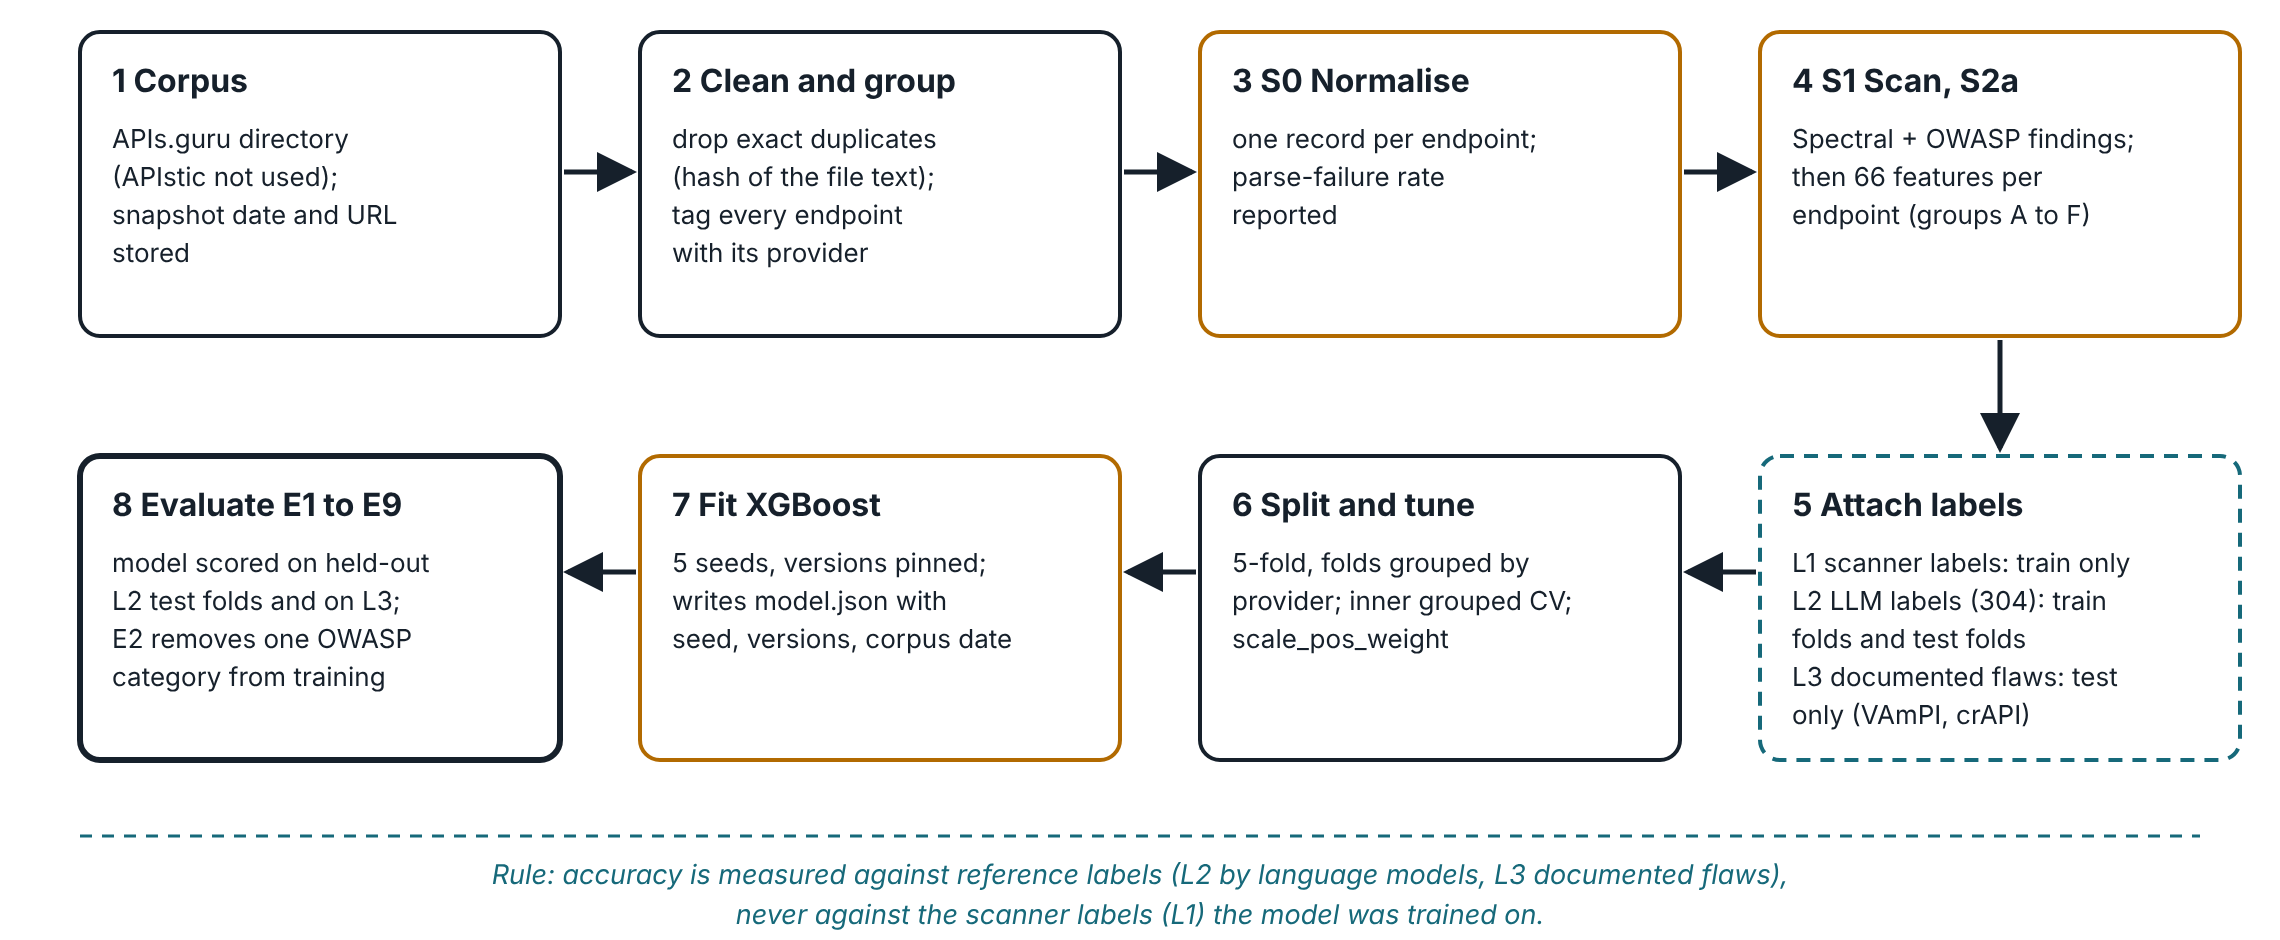
\includegraphics[width=0.92\textwidth]{methodology_v3.png}
\caption{Methodology in eight steps. The top row builds the dataset; the bottom row, read
right to left, labels it, trains the model and evaluates it. Amber marks shared code and the
model artefact; the dashed teal box marks the reference labels (L2, L3).}
\label{fig:method}
\end{figure*}

\subsection{Problem Statement and Label Definition}
\label{sec:m-prob}
Given an endpoint $e$ and its feature vector $x(e)\in\mathbb{R}^{d}$, learn a function $f$
whose output $r(e)=f(x(e))$ ranks endpoints by their relative risk of carrying a
security-relevant \emph{design} issue. The score is not calibrated
(Section~\ref{sec:m-gate}), so it orders endpoints but is not a probability. The label
$y(e)=1$ when the specification gives evidence of at least one
issue in an OWASP API Top 10 category that a specification can show~\cite{owasptop10}:
API1 (object-level authorisation), API2 (authentication), API3 (property-level exposure),
API4 (resource consumption), API5 (function-level authorisation), API8 (misconfiguration)
and API9 (improper inventory). API6, API7 and API10 rarely leave evidence in a specification;
they are recorded as ``not assessable'' and are never counted as negatives.

\subsection{Corpus Preparation}
\begin{enumerate}
\item \textbf{Snapshot.} Download the APIs.guru directory once and store the snapshot date,
the source URL of every file and the directory commit. All counts in the final report are
counts of this snapshot.
\item \textbf{Parse.} Run S0 on every file. Files that fail are logged with a reason and the
parse-failure rate is reported.
\item \textbf{De-duplicate.} Drop files whose text hash is already present. Exact hashes miss
near-copies, so the next step also protects against them.
\item \textbf{Group.} Give every endpoint a group identifier equal to its provider (the
directory name in APIs.guru, the repository in APIstic). Every split in this section is made
on groups, never on rows. Leakage between training and test data is a known cause of
over-optimistic results in machine-learning studies~\cite{kapoor}.
\item \textbf{Specification version.} The OWASP ruleset targets OpenAPI 3.x, so Swagger~2.0
files may receive fewer scanner labels for a reason unrelated to security. In the run reported here, scanner (L1)
training labels were taken from files of both versions, and the feature \texttt{is\_oas3} lets the model see the version, so a
version effect is possible. Training on OpenAPI~3.x files only is implemented (\texttt{-{}-oas3-train-only}) but was not run.
\end{enumerate}

\subsection{Labelling Protocol (T2)}
\label{sec:m-labels}
Three label sources are used, and each has a fixed job (Table~\ref{tab:labels}).

\begin{table}[!t]
\caption{What Each Label Source May Be Used For}
\label{tab:labels}
\centering
\footnotesize
\begin{tabularx}{\columnwidth}{L{1.5cm} L{1.5cm} L{1.2cm} Y}
\toprule
\textbf{Label} & \textbf{Made by} & \textbf{Train} & \textbf{Evaluate}\\
\midrule
L1 & Scanner & Yes & Never\\
L2 & Three LLM passes & Train folds only & Test folds\\
L3 & Documented flaws & No & Yes\\
\bottomrule
\end{tabularx}
\end{table}

\textbf{L1, weak labels.} $y_1(e)=1$ when the scanner reports at least one finding of
severity \texttt{error} or \texttt{warn} on $e$, ignoring rules that fire on more than 15\% of all
endpoints (a pilot scan showed that, without this, over 85\% of endpoints are flagged and the label carries no signal;
the ignored rules are listed in the dataset statistics file). These labels are cheap and noisy.
They fall in the weak-supervision setting described by Ratner \emph{et al.}~\cite{snorkel};
no label model is fitted, and the scanner output is used directly as noisy labels, for
training only.

\textbf{L2, reference labels.} A sample of 304 endpoints (plus a pilot of 32 that is
discarded) is drawn from the de-duplicated corpus at random within strata: flagged or not
flagged by the scanner, read method or write method, and small or large parent specification.
Because the sample is stratified, every reported metric is weighted by the inverse of the
sampling probability, so that it estimates the value on the whole corpus. \emph{The L2 labels
were produced by language models, not by people.} The procedure is:
\begin{enumerate}
\item Write a codebook with one decision rule per category of Section~\ref{sec:m-prob}.
\item Run a pilot of 32 endpoints, revise the codebook, and discard the pilot from the 304.
\item Three independent labelling passes (two Claude passes and one Codex pass) label all 304
endpoints without seeing scanner output, model scores or the sensitive-term lexicon. The
sheets given to the labellers contain only the endpoint, its specification excerpt and the codebook.
\item Report agreement before combining: pairwise Cohen's $\kappa$ was 0.49 to 0.58 and
Fleiss' $\kappa$ was 0.54, below the target of 0.6 that was set in advance. The codebook was
revised once after a pass misread an optional query-token rule; this is the only revision.
\item The final label is the majority vote of the three passes (62 of 304 endpoints, 20\%
positive); the category is the union of the categories of the passes that voted 1.
\end{enumerate}
Agreement between labellers does not show that they are right, and agreement between language
models is not independent evidence, so L3 is the external anchor. The agreement below target,
and the fact that no person checked the labels, are reported as threats to validity.

\textbf{L3, ground truth.} Endpoints of VAmPI and crAPI whose flaws are documented by their
authors (for crAPI, the 15 challenges listed by the OWASP project~\cite{crapichallenges}). The documented flaws are mapped to endpoints, and to OWASP API Top 10 2023 categories, by a language model that reads the project README and the handler source; no person reviewed this mapping. Many of these flaws live in the implementation and cannot be seen in a specification,
so L3 is reported twice: for all documented flaws, and for the subset visible at design level
(missing authentication, object-level access, excessive data in responses).

\subsection{Feature Extraction (S2a)}
\label{sec:m-feat}
S2a computes $d=66$ features in six groups (Table~\ref{tab:features}): A structural~(18),
B security scheme~(14), C data sensitivity~(7), D documentation~(11), E scanner-derived~(14)
and F context~(2). The implementation is a pure function with a fixed output order, no random
numbers, and no null values. Two choices need a justification.

\emph{Group C uses a lexicon.} It maps tokens of property names to weights 1 to 3: 3 for
credentials, payment and government identifiers, 2 for tokens, sessions and sensitive personal
attributes, 1 for ordinary personal data. Names are split on case changes and punctuation, so
\texttt{dateOfBirth} and \texttt{date\_of\_birth} match the same term. The list is compiled
from the OWASP API3:2023 examples and common personal-data categories, frozen before any
labelling, and is English only. Property names in other languages are not matched; this is a
stated limitation.

\emph{The provider is never a feature.} It is used only to group splits, so the model cannot
learn who wrote a specification.

\subsection{Training Algorithm (T4)}
Algorithm~\ref{alg:train} gives the procedure. The unit of every split is a provider. The
loss is the logistic loss of XGBoost~\cite{xgboost}. The positive class is a small minority,
so the positive-class weight is set from the training fold,
\begin{equation}
\texttt{scale\_pos\_weight}=\frac{N_{\text{neg}}}{N_{\text{pos}}},
\end{equation}
and models are compared with PR-AUC~\cite{saito}, F1 and the Matthews correlation
coefficient~\cite{chicco}, never accuracy.

The inner validation in Algorithm~\ref{alg:train} (line~7) uses the same labels as training:
$y_2$ where it exists and $y_1$ otherwise. Hyperparameter selection and early stopping are
therefore partly driven by scanner labels. This affects which model is chosen, not how it is
reported: every reported result is computed on test folds against the independently produced L2 and L3 labels only.

\begin{algorithm}[!t]
\caption{Grouped training and tuning (T4)}
\label{alg:train}
\footnotesize
\begin{algorithmic}[1]
\REQUIRE endpoints with features $x$, weak label $y_1$, reference label $y_2$ (where present), group $g$
\ENSURE model $f$, predictions on every test fold
\STATE split the groups into 5 folds $P_1,\dots,P_5$ with no group in two folds
\FOR{$i=1$ \TO $5$}
  \STATE $T\leftarrow$ endpoints with $g\notin P_i$;\; test set $\leftarrow$ endpoints with $g\in P_i$
  \STATE label of each $e\in T$ is $y_2(e)$ if it exists, else $y_1(e)$
  \STATE draw 30 hyperparameter settings at random (depth 3--8, learning rate 0.03--0.3, subsample, column sample, min.\ child weight, $\lambda$)
  \FOR{each setting}
    \STATE inner 3-fold cross-validation on $T$, again grouped by provider; train with early stopping on the inner validation part
    \STATE record mean PR-AUC
  \ENDFOR
  \STATE refit the best setting on all of $T$ with \texttt{scale\_pos\_weight} from $T$
  \STATE score the test set; for L2 and L3 endpoints keep the score and the reference label
\ENDFOR
\STATE repeat with 5 random seeds; report mean and interval over the seeds and folds
\STATE fit the final model on all groups and write \texttt{model.json} with seed, tool versions, schema versions, corpus date and selected $\tau$
\end{algorithmic}
\end{algorithm}

Four baselines are trained on the same feature table and scored on the same folds:
B0 the majority class; B1 the scanner itself (flagged is 1, optionally ordered by severity);
B2 logistic regression on standardised features; B3 random forest. A fifth baseline, B4, would ask a large language model for a risk score of each L2 endpoint at temperature~0. It is implemented (\texttt{e1\_llm\_baseline.py}) but was \textbf{not run}, so no language-model result is reported.

\subsection{Threshold and Gate Algorithm (S3)}
\label{sec:m-gate}
The threshold $\tau$ is chosen on validation folds, never on test folds. Validation labels
follow the same rule as in Algorithm~\ref{alg:train}: $y_2$ where it exists, $y_1$ otherwise.
Three operating points are reported: the $\tau$ that maximises F1 (the default), the smallest
$\tau$ with precision at least 0.9, and the largest $\tau$ with recall at least 0.9. The
default is written into the metadata of \texttt{model.json}. No post-hoc
calibration is applied, so that the score stays the logistic transform of the margin that SHAP
explains; a calibration curve is reported as a diagnostic.

As specified, the gate of~\eqref{eq:gate} rescans every endpoint, so a legacy API with old
problems would fail every build. The gate therefore counts only endpoints that are new or
changed relative to the base branch. Let $S_b$ and $S_h$ be the normalised base and head
specifications, let $\mathrm{key}(e)=(m,p)$ be the method and path of $e$, and let $h(e)$ be the hash
of the normalised record without file-identity fields. Then
\begin{multline}
\Delta(S_h,S_b)=\bigl\{\,e\in E(S_h)\;:\;\nexists\,e'\in E(S_b),\\
\mathrm{key}(e')=\mathrm{key}(e)\wedge h(e')=h(e)\,\bigr\},
\label{eq:delta}
\end{multline}
\begin{equation}
G_{\Delta}(S_h,S_b)=
\begin{cases}
1, & \bigl|\{\,e\in\Delta(S_h,S_b)\;:\;r(e)\ge\tau\,\}\bigr|>k,\\
0, & \text{otherwise.}
\end{cases}
\label{eq:gatedelta}
\end{equation}
The report still lists every endpoint in risk order and marks which ones were in scope. If no
base exists, every endpoint is new and~\eqref{eq:gatedelta} reduces to~\eqref{eq:gate}. A renamed path counts as a new endpoint. The endpoint
identifier of S0 cannot be used for matching, because it contains the specification hash and
changes whenever any line of the file changes. Matching costs $O(n)$ in the number of
endpoints.

\begin{algorithm}[!t]
\caption{Runtime scan with changed-endpoint gate (S0--S3)}
\label{alg:scan}
\footnotesize
\begin{algorithmic}[1]
\REQUIRE head specification $S_h$, optional base specification $S_b$, model $f$, threshold $\tau$, tolerance $k$
\ENSURE ranked report and exit code
\STATE $E_h\leftarrow$ S0$(S_h)$;\; $E_b\leftarrow$ S0$(S_b)$ if $S_b$ is given, else $\emptyset$
\STATE $A\leftarrow$ S1$(S_h)$ \COMMENT{findings attributed to endpoints}
\FORALL{$e\in E_h$}
  \STATE $x(e)\leftarrow$ S2a$(e,A(e),|E_h|)$;\; $r(e)\leftarrow f(x(e))$
\ENDFOR
\STATE $\Delta\leftarrow$ endpoints of $E_h$ that are new or changed relative to $E_b$ (all if $S_b$ is absent)
\STATE $n\leftarrow|\{e\in\Delta : r(e)\ge\tau\}|$
\STATE compute SHAP for every $e\in\Delta$ with $r(e)\ge\tau$ and for the 10 highest-scoring endpoints overall; write the report ranked by $r(e)$, marking $\Delta$
\RETURN $1$ if $n>k$, else $0$
\end{algorithmic}
\end{algorithm}

\subsection{Experiment Protocols}
All results use the same grouped folds, five seeds, and a provider-level bootstrap with 1{,}000
resamples for 95\% intervals. Two methods are compared on the same resamples.

\textbf{E1, accuracy against reference labels.} Algorithm~\ref{alg:train} is run and every model
is scored on the L2 endpoints of its test folds and on the L3 endpoints (VAmPI, crAPI), which are never in any training fold. The scanner is scored against the
same reference labels, so the comparison with the model is fair. Per-version results (OpenAPI~3.x
and Swagger~2.0) are reported separately.

\textbf{E2, rule hold-out.} This answers RQ2. Let $\mathcal{C}$ be the categories with at
least 20 positive endpoints in L2 and L3. For each $c\in\mathcal{C}$:
\begin{enumerate}
\item Remove from the training set every endpoint whose only findings are in category $c$.
\item Recompute every group-E feature from the findings with all category-$c$ findings
deleted, so that no feature carries any trace of $c$.
\item Train as in Algorithm~\ref{alg:train}.
\item On test folds, take the L2 endpoints whose reference categories include $c$ as
positives, and all other L2 endpoints as negatives (including positives of other categories). Report PR-AUC and recall at $\tau$.
\end{enumerate}
The reference for chance is the prevalence of $c$, and the reference for the best case is the
model trained with $c$ included. A category counts as \emph{generalised} when the lower end of
the 95\% interval of (PR-AUC minus prevalence) is above zero. The answer to RQ2 is the number
of categories that generalise out of $|\mathcal{C}|$, reported with its intervals. This
criterion is fixed here, before any result exists. Step~1 removes scanner findings only; L2 training endpoints whose reference label includes $c$ are not removed, so the held-out category is not fully unseen. This is a stated limitation of E2.

\textbf{E3, analyst effort and speed.} On the L2 sample, report P@$n$ for $n=5,10,20$ and the
number of findings read before all true positives are found, for the model ranking against the
scanner severity ranking, with $\tau$ swept over 0.1 to 0.9. Wall-clock time of S0 to S3 is
measured per component, 10 runs per specification, on specifications of 10 to 500 endpoints,
which tests the requirement that the runtime lane finishes in seconds.

\textbf{E4, external validity.} VAmPI and crAPI are scored by the final model, which never saw
them. Report the area under the ROC curve and the rank of each documented-flaw endpoint among
all endpoints. Schemathesis is run against the live VAmPI container (E9) to give an
independent dynamic finding set, which is compared with the ranking. OWASP ZAP 2.17.0 is run the same way (E10).
Both tools are used here only, never on the corpus.

\textbf{E5, ablation and explanation.} Remove each feature group in turn, and also remove
group E alone, and report the loss in PR-AUC. Report mean absolute SHAP values globally.
SHAP values for tree ensembles are computed exactly with TreeSHAP~\cite{treeshap}. They explain the raw
margin (log-odds), so the attributions sum to the margin minus the base margin, not to $r(e)$
itself. A \emph{text-inflation test} then checks whether the model can be gamed: for L2
negatives, set the group-D length features to the 90th percentile of the training data, change
nothing else, and report the mean score change and the share of endpoints that cross $\tau$.

\subsection{Experimental Setup}
\textbf{Data.} The APIs.guru directory holds 2{,}529 APIs with 108{,}837 endpoints before
de-duplication~\cite{apisguru}; counts after de-duplication and parsing are reported from the
frozen snapshot. VAmPI~\cite{vampi} and crAPI~\cite{crapi} are used for L3 and E4 only.

\textbf{Software.} Spectral and the ruleset are pinned exactly in \texttt{package.json}; the Python packages are listed with minimum versions in \texttt{requirements.txt}, and the versions actually used are written into each model file.
The feature schema (\texttt{s2a-1.0}) and the lexicon (\texttt{lex-1.0}) carry version labels
that are written into \texttt{model.json}, so a result can be traced to the exact code that
produced it. Every random seed is fixed and recorded.

\textbf{Hardware.} Training and all experiments run on one CPU workstation; the tabular
feature table does not need a GPU. Runtime in E3 is measured on a GitHub-hosted Ubuntu runner,
which is the reference deployment, and on the team's laptop, 10 runs per specification, with
the median and the range reported. Network time is excluded.

\textbf{Metrics.} PR-AUC, F1 and MCC for classification; P@$n$ and findings read
for analyst effort; milliseconds per specification for speed; mean absolute SHAP value for
explanation. All intervals are 95\% provider-level bootstrap intervals.

\textbf{Reproducibility.} The code, tests, feature schema and the figure scripts are kept in
one project folder, and the model file used for each reported table is committed with it: \texttt{model.json} for E1 to E4, and \texttt{model\_l2plus.json} (trained on the 608 reference labels of E7) for the packaged tool.

\subsection{Threats to Validity}
\textbf{Label noise.} L1 contains scanner errors; this is why it is never used for evaluation.
\textbf{Scanner shortcut.} Group~E features are derived from the same scanner output as the
L1 labels, so a model trained mostly on L1 can fit its training labels by copying group~E and
add little beyond the scanner. E5 measures this directly by removing group~E, and E2 tests it
category by category; if the shortcut dominates, that is reported as a finding.
\textbf{Small, model-labelled sample.} 304 endpoints give wide intervals, and the labels come from three language-model passes with Fleiss' $\kappa=0.54$ and a human audit of only 28 rows; intervals are reported rather
than hidden, and L3, whose flaws are documented by the VAmPI authors, is the external anchor (the flaw-to-endpoint mapping was done by a language model reading the handler source). \textbf{Specification versus implementation.} Design-level scores cannot see
implementation flaws; E4 measures the gap. \textbf{Corpus bias.} APIs.guru is dominated by
public commercial APIs and may not represent internal APIs. \textbf{Language.} The lexicon is
English only. \textbf{Tool drift.} A new Spectral or ruleset version changes L1 and the
baseline together, so versions are pinned. \textbf{Splits and tuning.} The five seeds differ only in how provider ties are broken: about 87\% of endpoints sit in the same fold under every seed, and the hyperparameters were tuned once under seed~0, so the spread over seeds understates uncertainty and the bootstrap intervals are the better guide. Precision at $k$ is not weighted by sampling probability. \textbf{Missing baseline.} The language-model baseline B4 was not run.

%==============================================================
\section{Results}
\label{sec:results}
All numbers come from the frozen run of 6 November 2026 on 80{,}974 endpoints from 665 providers,
evaluated on the 304 L2 endpoints (62 positive, 20\%). Intervals are 95\% provider-level bootstrap intervals.

\subsection{E1: Accuracy}
Table~\ref{tab:e1} gives the mean over five seeds (random forest: seed~0 only). The model is twice as good as always guessing the positive class in PR-AUC (0.21) and better than logistic regression in PR-AUC (difference 0.014 to 0.189), but not in F1 or MCC, where logistic regression is slightly higher. The random forest ties it on PR-AUC and has the highest ROC-AUC. It does \emph{not} beat the scanner alone: the PR-AUC difference to the scanner is $-0.20$ to $+0.16$, which includes zero.

\begin{table}[!t]
\caption{E1: Accuracy on L2 (mean of five seeds)}
\label{tab:e1}
\centering
\footnotesize
\begin{tabular}{lcccc}
\toprule
\textbf{Method} & \textbf{PR-AUC} & \textbf{ROC-AUC} & \textbf{F1} & \textbf{MCC}\\
\midrule
Always positive & 0.21 & 0.50 & 0.35 & 0.00\\
Scanner only (B1) & 0.47 & 0.69 & 0.43 & 0.26\\
Logistic regression & 0.33 & 0.72 & 0.47 & 0.30\\
Random forest & 0.42 & 0.75 & 0.44 & 0.27\\
XGBoost (APIGUARD) & 0.42 & 0.70 & 0.43 & 0.25\\
\bottomrule
\end{tabular}
\end{table}

\subsection{E2: Rule Hold-out (RQ2)}
Only 3 of the 10 categories had the 20 positives needed for a test. The model generalised on one of
them (Table~\ref{tab:e2}). The answer to RQ2 is therefore \textbf{1 of 3 tested categories}, and the other
seven could not be tested with this sample.

\begin{table}[!t]
\caption{E2: Held-out category, PR-AUC against prevalence}
\label{tab:e2}
\centering
\footnotesize
\begin{tabular}{lccccc}
\toprule
\textbf{Cat.} & \textbf{Pos.} & \textbf{Prev.} & \textbf{PR-AUC} & \textbf{ROC-AUC} & \textbf{Generalised}\\
\midrule
API2 & 54 & 0.18 & 0.22 & 0.57 & No\\
API3 & 24 & 0.10 & 0.15 & 0.50 & No\\
API5 & 34 & 0.09 & 0.37 & 0.91 & Yes\\
\bottomrule
\end{tabular}
\end{table}

\subsection{E3: Effort and Speed}
Fig.~\ref{fig:resa} shows the E1 curves, the threshold sweep and the run time. Ranking by model score did not reduce reviewer effort compared with scanner severity: precision at 5,
10 and 20 was 0.20, 0.30 and 0.20 for the model against 0.60, 0.40 and 0.55 for the scanner.
The precision and effort numbers use the out-of-fold scores of E1, so no test endpoint was seen in training. The best F1 over the threshold sweep was 0.47. Run time from S0 to S3 was 1.5 s for a 14-endpoint specification and 10.5 s for the largest (422 endpoints). The Spectral scan (S1) takes 1.4 s and 5.6 s, normalisation (S0) 0.07 s and 2.7 s, and the feature builder (S2a) 0.004 s and 2.1 s; the model (S2b) and the SHAP explanation (S2c) together take under 25 ms in every run.

\begin{figure*}[!t]
\centering
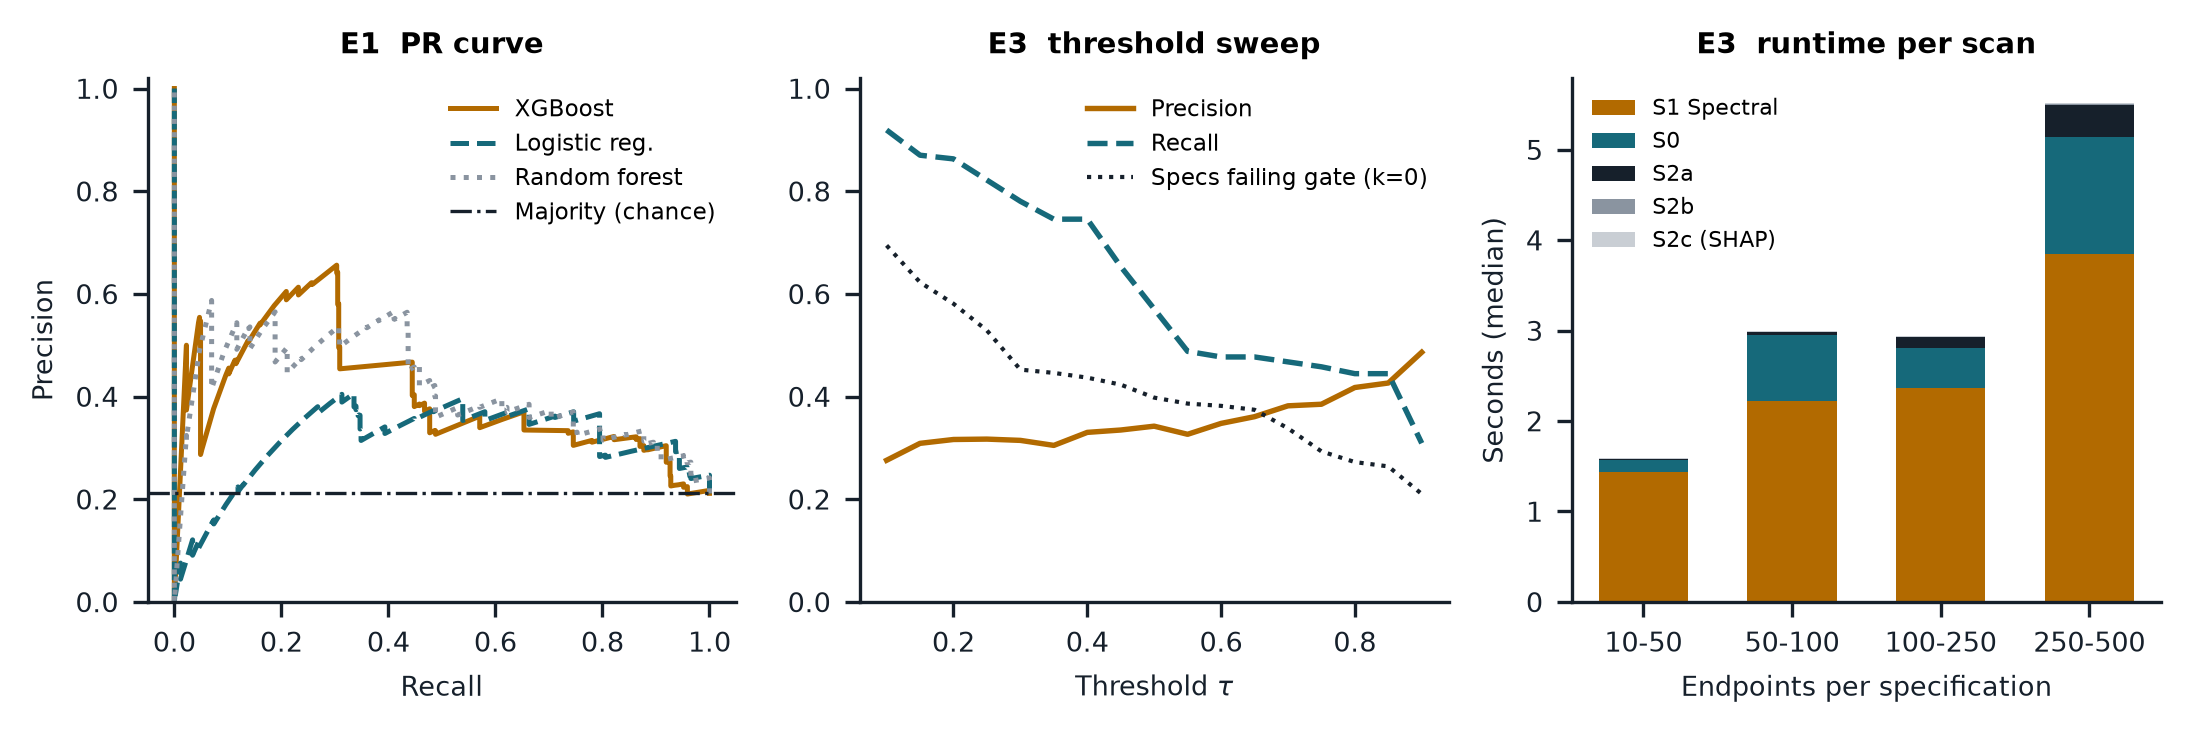
\includegraphics[width=0.95\textwidth]{results_a.png}
\caption{E1 precision--recall curves, E3 threshold sweep and E3 run time per scan, for the model trained on scanner labels.}
\label{fig:resa}
\end{figure*}

\subsection{E4: External Check on VAmPI and crAPI}
VAmPI has 14 endpoints, 10 with a documented flaw and 5 visible at design level. The ROC-AUC over all
flaws was 0.48 (PR-AUC 0.77 against a prevalence of 0.71) and over the design-visible flaws 0.22; the
design-visible endpoints ranked 8th to 12th of 14. crAPI has 44 endpoints, 15 mapped to the 15 challenges that
the OWASP project documents~\cite{crapichallenges}, and 3 of them visible at design level. The ROC-AUC over
all flaws was 0.39 (PR-AUC 0.30 against a prevalence of 0.34) and over the design-visible flaws 0.16; those
three endpoints ranked 31st, 38th and 40th of 44.

This is a negative result on both applications: the model does not rank flawed endpoints above others, and it
is worse than a random ranking on the flaws that a specification can show. The ranked tables show why. The
highest scores go to authentication and write endpoints that the scanner flags many times, and the lowest scores
go to read (GET) endpoints that declare no authentication, which are the clearest design-level flaw
(\texttt{/users/v1/\_debug} in VAmPI, \texttt{receive\_report} in crAPI). A model trained to agree with scanner
and language-model labels inherits whatever they under-weight. Two cautions apply: each application is small, so
no interval is given, and the flaw-to-endpoint mapping was made by a language model from the project documentation and handler
source (Section~\ref{sec:m-prob}). The dynamic comparison with Schemathesis is reported in Section~\ref{sec:e9} for VAmPI only; OWASP ZAP was run on VAmPI and on Damn Vulnerable RESTaurant (Sections~\ref{sec:e10} and~\ref{sec:e13}); crAPI needs Docker and was not tested dynamically. Section~\ref{sec:e6} tests a likely cause.

\subsection{E5: Ablation and Explanation}
Removing the structural group A cost the most (PR-AUC 0.44 to 0.30). Removing B cost 0.03, and removing C, D, E or F did not lower it (0.46, 0.44, 0.44 and 0.48), so the data-sensitivity group C, which was meant to capture what a rule cannot see, carries no measurable signal in this sample.
Mean absolute SHAP was highest for the security-scheme group B, then scanner-derived E and structural A.
The text-inflation test did not game the model: setting description lengths to the 90th percentile moved
the mean score by $-0.011$ and only 0.7\% of negatives crossed $\tau$.

\subsection{E6: Training Only on the Reference Labels}
\label{sec:e6}
The E4 failure has a likely cause in how E1 to E4 were trained. About 81{,}000 of the training labels are scanner (L1) labels,
and L1 ignores every rule that fires on more than 15\% of endpoints. That list includes \texttt{owasp:api2:2023-read-restricted},
the rule for a read endpoint without authentication. So the model was taught that such endpoints are normal. The reference labels
say otherwise: among the 304 L2 endpoints, 47\% of those with no security requirement are positive against 5\% of those with one.
E6 therefore trains the model \emph{only} on the 304 reference labels, with the same provider-grouped five-fold protocol and five seeds,
and compares it with the scanner on the same test folds. Only this one variant was run. It was motivated by the E4 result and by the
label rates above, so E4 is no longer a clean external test for it; the E6 test folds are, because they are out-of-fold.

\begin{table}[!t]
\caption{E6: Trained on L2 only, out-of-fold on L2 (mean of five seeds)}
\label{tab:e6}
\centering
\footnotesize
\begin{tabular}{lcccc}
\toprule
\textbf{Method} & \textbf{PR-AUC} & \textbf{ROC-AUC} & \textbf{F1} & \textbf{MCC}\\
\midrule
Scanner only (B1) & 0.47 & 0.69 & 0.43 & 0.26\\
Logistic regression & 0.47 & 0.81 & 0.52 & 0.38\\
XGBoost, L2 only & 0.48 & 0.80 & 0.52 & 0.39\\
\bottomrule
\end{tabular}
\end{table}

On the seed-averaged out-of-fold scores the ROC-AUC of XGBoost is 0.84 against 0.69 for the scanner, and the
provider-level bootstrap interval of the difference is $+0.01$ to $+0.33$, which excludes zero only narrowly.
The PR-AUC difference is $-0.20$ to $+0.37$ and includes zero. On the two external applications the
L2-only model gave ROC-AUC 0.86 on VAmPI against 0.48 before (design-visible flaws 0.72 against 0.22), and 0.39 on crAPI
against 0.39 before (design-visible flaws 0.63 against 0.16). So it fixed VAmPI and not crAPI. The effort measures of E3 are repeated with the out-of-fold scores of this model in Section~\ref{sec:e8}. Because the labels are language-model labels, E6 measures agreement
with those labels; the two applications are the only evidence that does not depend on them.

\subsection{E7: Doubling the Reference Labels}
\label{sec:e7}
To test whether label count is the limit, 304 further endpoints were labelled by one language-model pass with the same
codebook and the same stratified draw, excluding every endpoint of the test sample and the pilot (67 positives, 22\%). They are used for
training only; the test set is still the original 304 endpoints, scored out-of-fold, and the extra endpoints of a provider that is in a
test fold are not used for that fold. Because it is a single pass, no agreement score exists for these labels.

\begin{table}[!t]
\caption{E7: XGBoost on the original test set, mean of five seeds}
\label{tab:e7}
\centering
\footnotesize
\begin{tabular}{lcccc}
\toprule
\textbf{Training labels} & \textbf{PR-AUC} & \textbf{ROC-AUC} & \textbf{F1} & \textbf{MCC}\\
\midrule
Scanner only (B1) & 0.47 & 0.69 & 0.43 & 0.26\\
L2 only (E6, 304) & 0.48 & 0.80 & 0.52 & 0.39\\
L2 + extra (608) & 0.52 & 0.81 & 0.51 & 0.40\\
\bottomrule
\end{tabular}
\end{table}

Doubling the labels did not change the result measurably: the difference to E6 is $-0.16$ to $+0.22$ in PR-AUC and $-0.05$ to $+0.05$
in ROC-AUC. Against the scanner, the seed-averaged ROC-AUC is 0.84 against 0.69, with a difference of $+0.03$ to $+0.32$, and the PR-AUC
difference is $-0.11$ to $+0.34$. On the external applications the model trained on 608 labels reached ROC-AUC 0.79 on VAmPI and
0.37 on crAPI. So more labels of this kind did not fix crAPI, and label count alone is not the limit; label quality and coverage of the
flaws that crAPI contains (mostly implementation flaws) are more likely limits.

\subsection{The Packaged Tool}
The command line was packaged as a single Windows executable with PyInstaller (about 410 MB, because it carries XGBoost and SHAP).
It needs Node.js and the Spectral package next to it for the scanner step. Run on VAmPI (14 endpoints) and crAPI (44 endpoints)
with \texttt{model\_l2plus.json} and the model's own threshold $\tau=0.53$, it printed the ranked endpoints with their top SHAP reasons
and the scanner rules that fired, and ended with ``GATE: FAIL'' and exit code 1 on both, the expected verdict for applications built to
be vulnerable. On one small hand-written clean specification (two endpoints, bearer authentication everywhere, no sensitive fields, \texttt{demo/specs/clean\_openapi3.yaml}) the gate passed with both models (highest score 0.16). This is one example and not a measured false-alarm rate, which is known only from the E1 and E3
measurements above.

\subsection{E8: Scanner and Model Combined}
\label{sec:e8}
E3 asked whether the model ranks findings better than the scanner and the answer was no. The design places the model \emph{after} the scanner, so
E8 tests the combination: the score is the mean of the percentile rank given by the scanner (severity, then rule count) and the percentile rank given by
the model. This one setting was fixed in advance and no weight was tried. All scores are out-of-fold on the original 304 test endpoints, averaged over the five seeds;
precision at $k$ and the findings read before the last true positive follow the definitions of E3.

\begin{table}[!t]
\caption{E8: Ranking on the test set (model trained on the 608 reference labels of E7)}
\label{tab:e8}
\centering
\scriptsize
\begin{tabular}{lcccccc}
\toprule
\textbf{Ranking} & \textbf{PR-AUC} & \textbf{ROC} & \textbf{P@5} & \textbf{P@10} & \textbf{P@20} & \textbf{Read}\\
\midrule
Scanner only & 0.47 & 0.69 & 0.60 & 0.40 & 0.55 & 272\\
Model only & 0.52 & 0.81 & 0.64 & 0.60 & 0.57 & 279\\
Scanner + model & 0.55 & 0.80 & 0.88 & 0.76 & 0.66 & 245\\
\bottomrule
\end{tabular}
\end{table}

Against the scanner the combination gains $+0.03$ to $+0.30$ in PR-AUC and $+0.05$ to $+0.24$ in ROC-AUC (provider-level 95\% intervals, both excluding zero), and a reviewer
who reads the top 10 finds 7.6 true positives on average in expectation against 4.0 (precision 0.76 against 0.40). Against the model alone the differences are not
significant ($-0.13$ to $+0.19$ in PR-AUC). The model trained only on 304 labels (E6) gives a smaller gain whose PR-AUC interval includes zero ($-0.16$ to $+0.27$). Two caution points: this is the best of the combinations
reported here only in the sense that it is the one we specified, but the two training policies and the two metrics make four comparisons, so the intervals should be read as indicative; and precision at $k$ has no interval because it is computed on a single sample of 304 endpoints with 62 positives. The packaged command line gates on the model score alone; this scanner-plus-model ranking is not implemented in it.

\subsection{E9: Dynamic Check with Schemathesis on VAmPI}
\label{sec:e9}
To get one finding set that does not come from our labels, Schemathesis 4.33.2 (official Docker image) was run against a live VAmPI container
(freshly populated database, a valid login token, all checks, up to 50 examples per operation, 805 test cases, 14 of 14 operations). It reported 18 unique failures, on 8 of the 14 scored endpoints and on 3 OPTIONS operations that the model does not score.
Schemathesis checks server errors, schema conformance, undocumented responses and state handling; it has no check for logic flaws such as broken object-level authorisation.
Two readings of its output were prepared before it was compared with the model: \emph{any} failure on an operation (8 of the 14 endpoints), and \emph{strict} failures only (server error, response
violating the schema, or created resource not found: 2 endpoints, \texttt{PUT /users/v1/\{username\}/password} and \texttt{GET /books/v1/\{book\_title\}}).

The agreement is weak. Against the 10 documented flaws, Schemathesis flags 5 endpoints under the \emph{any} reading (recall 0.50) and 2 under the \emph{strict} reading (recall 0.20), while
the four endpoints above the gate threshold of the model trained on 608 labels are all documented flaws (\texttt{GET /users/v1/\{username\}}, \texttt{POST /users/v1/login}, \texttt{POST /users/v1/register}, \texttt{GET /users/v1/\_debug}).
Taking the dynamic finding as the label, the model score gives a ROC-AUC of 0.25 (\emph{any}) and 0.27 (\emph{strict}) over 14 endpoints, that is no agreement, and slightly below chance. The two tools find different things:
the model ranks endpoints whose design resembles known OWASP risks, whereas Schemathesis finds endpoints that misbehave under malformed input. The endpoint the model ranks first (\texttt{GET /users/v1/\{username\}}) is not flagged by Schemathesis at all.
With 14 endpoints and 2 to 8 positives this is an observation, not a test. It means the dynamic tool cannot confirm the ranking, and it also cannot refute it, because it does not look for the flaws that the ground truth lists.

\subsection{E10: OWASP ZAP on VAmPI}
\label{sec:e10}
OWASP ZAP is the real, widely used OWASP scanner, so it is the baseline the demo should be compared with. ZAP 2.17.0 was run with its Automation Framework against a live VAmPI
in vulnerable mode (the same specification imported, 14 operations, passive scan, active scan), once without a token and once with a valid bearer token.
ZAP raised four alert types: one High (SQL injection on \texttt{GET /users/v1/\{username\}}, low confidence),
two Low that are header hygiene (server version banner, missing \texttt{X-Content-Type-Options}) on up to seven endpoints, and one informational. Two readings were fixed before scoring, as in E9:
\emph{medium or higher} (a finding about the application) and \emph{low or higher} (which adds the header alerts, unrelated to the documented flaws).

\begin{table}[!t]
\caption{ZAP, Spectral and APIGUARD against the L3 ground truth of VAmPI (14 endpoints, 10 documented flaws).}
\label{tab:e10}
\centering
\footnotesize
\begin{tabular}{lrrrrr}
\toprule
\textbf{Reading} & \textbf{Flagged} & \textbf{TP} & \textbf{FP} & \textbf{Recall} & \textbf{Prec.}\\
\midrule
ZAP medium or higher & 1 & 1 & 0 & 0.10 & 1.00\\
ZAP low or higher (headers) & 7 & 6 & 1 & 0.60 & 0.86\\
Spectral OWASP (S1 alone) & 14 & 10 & 4 & 1.00 & 0.71\\
APIGUARD score $\geq\tau$ & 2 & 2 & 0 & 0.20 & 1.00\\
APIGUARD top 10 by score & 10 & 7 & 3 & 0.70 & 0.70\\
\bottomrule
\end{tabular}
\end{table}

Read this table with care. ZAP's medium-or-higher reading finds one documented flaw endpoint (\texttt{GET /users/v1/\{username\}}), which APIGUARD also ranks high. Its low reading reaches six flaw endpoints,
but the alert is a header issue that every endpoint of this server has, so the match is coincidence, not detection. Spectral flags all 14 endpoints (document-level findings are attributed to every endpoint), so its recall of 1.00 says nothing.
APIGUARD (model \texttt{model.json}) puts 7 of the 10 flaws in its top 10 and 2 above $\tau$; the ROC-AUC of its score is 0.48 over all 14 endpoints, and that of ZAP's maximum risk is 0.69, both uninformative at this size (prevalence 0.71).
Of the ten flaw endpoints, APIGUARD's top 10 covers six that ZAP does not (for example \texttt{GET /users/v1/\_debug}, which returns every user's password), both cover one, and neither covers three. The tools see different things: ZAP sends traffic and found an injection that the specification does not show, APIGUARD reads the design and
sees missing authentication and exposed fields that ZAP's default rules do not test. Limits: one application, 14 endpoints; default ZAP policy with a static token; crAPI needs Docker and was not run; ZAP's JSON reports are in \texttt{results/zap/}.

\subsection{E11: LLM Checker with a Random Human Audit}
\label{sec:e11}
\texttt{experiments/e11\_audit\_loop.py} runs the lane of Section~\ref{sec:feedback} on the real L2 study. The checker accepted 228 of the 304 verdicts (75\,\%) because all three passes agreed, and dropped 76 split votes. Of the accepted verdicts 38 are positive.
The seeded audit sample (seed 20261117) holds 23 endpoints, 4 of them positive by the checker. The blind sheet is \texttt{results/audit/L2\_audit\_sheet.csv} and the person labels it in \texttt{AUDIT\_TOOL.html} (about ten minutes).
\textbf{Result.} One person (a team member, working alone and blind to the checker's verdicts) labelled the 23 rows, then 5 further rows drawn at random from the same accepted verdicts (1 checker-positive). The person and the checker agreed on all 28 (agreement 1.00, Wilson 95\,\% interval 0.88 to 1.00, Cohen's $\kappa=1.00$), so the batch is accepted and no label was changed. Read this with care: 28 rows is a small sample, only 5 are checker-positive, the person has no specialist security training, and the audit can only catch a checker whose error rate is high (it would have quarantined a checker with 30\,\% error 86\,\% of the time, but one with 10\,\% error only 7\,\% of the time). The result says the unanimous verdicts are consistent with one person's reading on a random sample; it does not show the checker is correct. The audit files are \texttt{results/audit/}.

\subsection{E12: A Wider Corpus}
\label{sec:corpus-ext}
APIs.guru is mostly public vendor and cloud APIs. To add variation, \texttt{tools/fetch\_extended.py} downloaded specifications from 50 further GitHub repositories chosen for
different kinds of author and domain: telecom (CAMARA), banking and payments, communication and SaaS vendors, DevOps and observability products, backend-as-a-service tools, IoT, generator test suites with edge-case specifications, and vulnerable-by-design applications.
Every file is stored with its repository, commit, path and hash (\texttt{corpus\_ext/manifest.*.jsonl}). Of 436 files, 17 failed to parse (3.9\,\%, against 0.12\,\% for APIs.guru) and one failed in the scanner. Specifications whose operations overlap an APIs.guru file by Jaccard 0.5 or more
were dropped as near-copies (45 specifications, 2{,}139 endpoints), leaving 368 specifications, 9{,}741 endpoints and 25 provider groups. Of these, 78\,\% are OpenAPI 3.x (the rest Swagger~2.0). The two corpora differ in composition (Table~\ref{tab:ext}): the added endpoints more often declare no security (62\,\% against 34\,\%),
are fewer per specification and use plain-HTTP servers about half as often.

\begin{table}[!t]
\caption{APIs.guru and the added sources (after near-copy removal).}
\label{tab:ext}
\centering
\footnotesize
\begin{tabular}{lrr}
\toprule
 & \textbf{APIs.guru} & \textbf{Added}\\
\midrule
Specifications & 2{,}493 & 368\\
Endpoints & 80{,}974 & 9{,}741\\
Provider groups & 665 & 25\\
Median endpoints per spec. & 8 & 5\\
No security requirement & 34.0\,\% & 62.3\,\%\\
Server on plain HTTP & 23.5\,\% & 11.8\,\%\\
Scanner (L1) positive rate & 28.4\,\% & 41.0\,\%\\
\bottomrule
\end{tabular}
\end{table}

\textbf{Transfer test.} The scanner-blind model (feature groups A--D and F, trained on APIs.guru L1 labels, five seeds) was applied to the added endpoints, which it never saw. Against their L1 labels it reaches ROC-AUC 0.77 (95\,\% provider-bootstrap interval 0.65 to 0.96) and PR-AUC 0.60 (0.29 to 0.98) at prevalence 0.41,
against ROC-AUC 0.95 and PR-AUC 0.88 on held-out APIs.guru providers (prevalence 0.08). The model therefore transfers, but loses accuracy on new kinds of API. It does best on open-source products (ROC-AUC 0.91) and generator test suites (0.87),
and worst on vendor APIs (0.82 ROC-AUC, PR-AUC 0.40 at prevalence 0.09); OpenAPI 3.x endpoints score 0.78 and Swagger~2.0 endpoints 0.86. The intervals are wide because there are only 25 provider groups. This measures how well design features reproduce scanner findings on unseen sources; it is not a security-quality claim, since no L2 or L3 labels exist for these endpoints.

\subsection{E13: ZAP and APIGUARD on a Second Application}
\label{sec:e13}
E10 used one application, so a second was added: Damn Vulnerable RESTaurant (DVR)~\cite{dvr}, a FastAPI training application with 21 operations in its OpenAPI document. Its flaws are documented by its own vulnerability tests, so no labels were made by hand.
Six of the 21 operations are documented as flawed: \texttt{GET /healthcheck} (technology header), \texttt{DELETE /menu/\{item\_id\}} (no authorisation), \texttt{PUT /profile} (IDOR), \texttt{PUT /users/update\_role} (privilege escalation), \texttt{PUT /menu} (SSRF) and \texttt{GET /admin/stats/disk} (command injection).
Two further documented flaws are hidden endpoints that are not in the OpenAPI document and so cannot be scored. The API categories in the label file are our own assignment, and two operations are marked design-visible (no authorisation check, role field in the body) by our judgement; the scores below do not use them.
ZAP 2.17.0 was run as in E10, with no token, a customer token and an employee token, and the reports were combined; ZAP never held a chef token (its password is random at start-up).

\begin{table}[!t]
\caption{ZAP, Spectral and APIGUARD against the documented flaws of DVR (21 operations, 6 flaws).}
\label{tab:e13}
\centering
\footnotesize
\begin{tabular}{lrrrrr}
\toprule
\textbf{Reading} & \textbf{Flagged} & \textbf{TP} & \textbf{FP} & \textbf{Recall} & \textbf{Prec.}\\
\midrule
ZAP medium or higher & 5 & 1 & 4 & 0.17 & 0.20\\
ZAP low or higher (headers) & 14 & 4 & 10 & 0.67 & 0.29\\
Spectral OWASP (S1 alone) & 21 & 6 & 15 & 1.00 & 0.29\\
APIGUARD score $\geq\tau$ & 5 & 1 & 4 & 0.17 & 0.20\\
APIGUARD top 6 by score & 6 & 2 & 4 & 0.33 & 0.33\\
\bottomrule
\end{tabular}
\end{table}

The result is weak for both tools. ZAP's medium-or-higher reading finds only \texttt{PUT /profile}; its other four High alerts (SQL injection on \texttt{/reset-password}, \texttt{/reset-password/new-password}, \texttt{/orders} and \texttt{PATCH /profile}) are counted as false positives here, but we did not confirm them by hand.
Their evidence is a server error after a quote character or a changed response to \texttt{OR 1=1}, and the application uses an ORM for these routes, so they are probably false alarms. They might also be real undocumented flaws, which a documented-flaw ground truth cannot tell.
APIGUARD ranks \texttt{GET /admin/stats/disk} highest of the flawed operations and \texttt{GET /healthcheck} sixth; its other four top-ranked operations are authentication routes that are not flawed. ZAP found the flaw that APIGUARD missed (\texttt{PUT /profile}) and APIGUARD found two that ZAP missed
(the command injection, which ZAP could not reach without a chef token, and the header, which ZAP reports only as a low alert). Three flaws were found by neither (\texttt{DELETE /menu/\{item\_id\}}, \texttt{PUT /menu}, \texttt{PUT /users/update\_role}), which are the authorisation and role flaws.
The ROC-AUC of APIGUARD's score is 0.62 and that of ZAP's maximum risk is 0.47 (prevalence 0.29); with six positives the difference is not meaningful. Across E10 and E13 the pattern is the same: the two tools find different flaws, neither dominates, and each misses most authorisation flaws.
Limits: two applications, both small; documented flaws only; default ZAP policy; crAPI still not run (it needs Docker). Reports and scoring are in \texttt{results/e13\_zap.json}.

\subsection{E14: Trying to Improve the Model}
\label{sec:e14}
E10 and E13 showed that the model misses authorisation, role and injection flaws, so eight pattern features were added (group G, schema 1.1) after those misses were known. On the 304 reference endpoints (provider-grouped five-fold cross-validation, three seeds, fixed XGBoost parameters, same folds) the PR-AUC rose from $0.42\pm0.03$ to $0.48\pm0.01$, with a 95\,\% provider-bootstrap interval of $-0.11$ to $+0.14$ for the difference, so the gain is not distinguishable from noise. A threshold rule fixed in advance (the highest value with out-of-fold recall of at least 0.60) gave $\tau=0.90$. Scored once on VAmPI and DVR, the new model did not improve (ROC-AUC 0.48 to 0.40 and 0.62 to 0.50, both within noise); DVR declares an authentication scheme on every operation, so a specification-only model cannot see that the server does not check it. The model was not adopted and nothing was tuned on the test applications; E15 is a separate, later revision. Files: \texttt{results/e14\_improve.json}, \texttt{results/e14b\_tau.json}.

\subsection{E15: Model v3}
\label{sec:e15}
The earlier experiments pointed to three causes of weak ranking. The model trained on scanner labels can only copy the scanner (E1--E4); the context group F hurt in the ablation (E5); and S1 attached every document-level finding (components, security schemes, servers) to every endpoint of a specification, so most endpoints of one specification carried the same rules and group E could not tell them apart. Model v3 changes four things and nothing else:
(i)~it is trained only on the 608 reference labels of E7, with scanner output used as features, never as labels;
(ii)~group E counts only the findings on the endpoint's own operation or path item, and document-level findings are kept out (they were also tried as a separate group S);
(iii)~group F is removed;
(iv)~a new group H of fourteen flaw-pattern features is added: an object identifier in the path of a read, update or delete (and the same for user-like objects and without authentication), admin and debug words in the path, a write without authentication, privilege, ownership or money fields that the request body can set, a URL-valued field, an authentication endpoint with and without a rate limit, a secret in the success response, an unpaged collection and a numeric path identifier (schema s2a-3.0, \texttt{features\_v3.py}).
Like group G (E14), group H was written after the misses of E10 and E13 were known; every variant therefore uses the same fixed XGBoost settings (depth 3, learning rate 0.05, early stopping) and nothing was tuned.

\textbf{Protocol.} The test set is the 304 original reference endpoints, with provider-grouped five-fold cross-validation over five seeds; the other 304 reference endpoints are always in training, except those from a provider in the test fold. Scores are weighted as in E1 and all variants share the same folds; the harness reproduces the earlier figures (scanner 0.47 as in E1, v1 features 0.52 as in E8). For the external check each variant is trained on all 608 labels.

\begin{table}[!t]
\caption{E15: Model variants on the same folds (mean of five seeds). External columns are ROC-AUC.}
\label{tab:e15}
\centering
\scriptsize
\begin{tabular}{lccccc}
\toprule
\textbf{Variant} & \textbf{PR-AUC} & \textbf{ROC} & \textbf{P@10} & \textbf{VAmPI} & \textbf{crAPI}\\
\midrule
Random & 0.21 & 0.50 & -- & 0.50 & 0.50\\
Scanner only (B1) & 0.47 & 0.69 & 0.40 & 0.51 & 0.61\\
v1 features (E8 model) & 0.52 & 0.81 & 0.70 & 0.82 & 0.37\\
+ per-endpoint E, no F & 0.51 & 0.80 & 0.72 & 0.85 & 0.40\\
\textbf{+ group H (v3)} & \textbf{0.62} & \textbf{0.85} & 0.76 & 0.80 & 0.40\\
v3 + document-level S & 0.56 & 0.82 & 0.82 & 0.78 & 0.41\\
v3 without scanner features & 0.63 & 0.83 & 0.82 & 0.82 & 0.53\\
\bottomrule
\end{tabular}
\end{table}

\textbf{Result.} Table~\ref{tab:e15} gives the variants. Per-endpoint attribution and the removal of F leave the score unchanged; the gain comes from group H. Against the scanner, v3 gains $+0.01$ to $+0.43$ in PR-AUC and $+0.05$ to $+0.35$ in ROC-AUC (provider-level 95\,\% intervals, both excluding zero); it is the first single model in this paper whose PR-AUC interval against the scanner excludes zero. Against the v1 features trained on the same labels the gain is $-0.07$ to $+0.26$ in PR-AUC and $-0.005$ to $+0.10$ in ROC-AUC, so it is better on average but not significantly. Combining v3 with the scanner as in E8 adds nothing (PR-AUC 0.60), document-level findings (S) lower the score, and removing the scanner features gives a similar score, so most of the signal is in the design features. With the rule fixed in E14 (the highest threshold with out-of-fold recall of at least 0.60), $\tau=0.60$, with precision 0.56 and 72 of the 304 endpoints flagged. SHAP ranks the security-scheme features first; \texttt{h\_write\_noauth} is fourth.

\textbf{Limit.} On crAPI v3 is still below chance (ROC-AUC 0.40, against 0.61 for the scanner); on VAmPI it reaches 0.80. The cause is in the labels: of the 129 positive reference labels, 117 are endpoints without authentication, and only 12 of the 377 authenticated endpoints are positive. The model therefore learns that a missing login means risk. Every crAPI endpoint is authenticated and its flaws are authorisation and logic flaws, so v3 ranks its public login and sign-up operations first. New features cannot fix this; it needs labels in which an authenticated endpoint can be risky. A codebook for that (one question per OWASP category; public-by-design endpoints not risky for lacking a login) is in \texttt{results/v3/CODEBOOK\_v3.md}. v3 was not scored on DVR. The packaged tool now loads v3 by default (\texttt{models/model\_v3.json}, $\tau=0.60$); on VAmPI it flags four endpoints, all documented flaws. Files: \texttt{experiments/v3/}, \texttt{results/v3/}.

\subsection{Discussion and Limitations}
The honest conclusion has two parts. Trained on scanner labels (E1 to E4), APIGUARD matches the scanner at similar accuracy and the same cost, generalises to one
unseen category, and does not beat the scanner. Trained only on the reference labels (E6), it beats the scanner on ROC-AUC (difference $+0.01$ to $+0.33$) and on F1 and MCC, but not
significantly on PR-AUC, and it still ranks crAPI flaws no better than chance, even with twice as many reference labels (E7). Combined with the scanner (E8), it ranks better than the scanner alone in both PR-AUC and ROC-AUC, which is the use the design intends. Four things limit this. (i)~The reference labels were produced by
language models, with Fleiss' $\kappa=0.54$ and a human check only of 28 rows (a random 23-row sample plus 5 extra) of the accepted verdicts (Section~\ref{sec:e11}), so noise in them caps every score. (ii)~The test set holds only 62 positives (129 across all 608 reference labels),
so most categories were untestable. (iii)~L1 labels are the scanner's own, so a model trained on them can at best
approximate it. (iv)~On the two external applications the scanner-trained model ranked flawed endpoints no better than chance (E4), and the L2-trained model did well on VAmPI but not on crAPI (E6), so the claim is limited to the corpus labels, and the dynamic comparison covers VAmPI (Schemathesis, E9; ZAP, E10) and Damn Vulnerable RESTaurant (ZAP, E13). The added sources (E12) are few providers with wide intervals and carry scanner labels only. A larger, human-labelled sample and more runnable vulnerable-by-design applications would be the first things to add. The revised model v3 (E15) is the strongest result: it beats the scanner on both PR-AUC and ROC-AUC with intervals that exclude zero, but it shares the label limit above, which is why it still fails on crAPI.

\textbf{Sensitivity to the labels.} The analysis was repeated with an earlier key made from two passes
plus an adjudication (46 positives). E1 was similar (XGBoost 0.46, scanner 0.43, difference $-0.21$ to $+0.30$).
E2 changed: with that key only API2 and API5 had enough positives, and both generalised (2 of 2).
So the E2 answer depends on the label key. API5 generalises under both keys; API2 does not under the majority key.
We report the majority-vote result as the main one, because it was fixed before the sensitivity run, and
treat RQ2 as unresolved at this sample size.

%==============================================================
\section{Conclusion}
This paper has specified the APIGUARD system model: three lanes separated by when they
run and how far they are trusted, a runtime path of four components from specification to CI
exit code, an offline path that produces the model artefact those components load, and a
feedback path that returns LLM-checked verdicts, audited at random by a person, to the label store without ever closing a loop into
the model. The notation and the gate rules in~\eqref{eq:scored}, \eqref{eq:gate}
and~\eqref{eq:gatedelta} fix what the implementation must compute, and the interface contracts
fix what each component must guarantee. Section~\ref{sec:method} turns this model into the proposed methodology and algorithm: the label
protocol that keeps scanner labels out of every evaluation, the feature extraction, the grouped
training procedure, a gate that judges only new or changed endpoints, and the protocol for the
rule hold-out experiment that the whole design rests on. The experiments of Section~\ref{sec:results} show that, trained on scanner labels, the model matches but does not beat the scanner and generalises in the rule hold-out for one of three testable categories. Trained on language-model reference labels it ranks better by ROC-AUC, and combined with the scanner it ranks better on PR-AUC and ROC-AUC, but it does not reliably rank the flaws of crAPI. The revised model v3 (E15), with per-endpoint scanner findings and flaw-pattern features, beats the scanner on both PR-AUC (0.62 against 0.47) and ROC-AUC (0.85 against 0.69). All reference labels were produced by language models, and they mark almost only unauthenticated endpoints as risky, so these results measure agreement with those labels; relabelling with a codebook that lets authenticated endpoints be risky, on a sample drawn from more providers, is the main next step.

%==============================================================
% If you prefer BibTeX on Overleaf, delete the thebibliography block
% below and uncomment these two lines (refs.bib is included):
% \bibliographystyle{IEEEtran}
% \bibliography{refs}

\section*{Use of Generative AI}
Generative AI tools (Claude and Codex) were used to help write the code, run the experiments, produce the reference labels (Section~\ref{sec:m-labels}) and draft and edit this report. The authors checked the results and take full responsibility for the content; every number in this paper comes from the code and result files in the project repository.

\def\UrlBreaks{\do\/\do-\do.}
\begin{thebibliography}{99}
\bibitem{apistic}
S.~Serbout and C.~Pautasso, ``APIstic: A large collection of OpenAPI metrics,'' in
\emph{Proc. 21st Int. Conf. Mining Software Repositories (MSR)}, Lisbon, Portugal, 2024,
pp.~265--277, doi: 10.1145/3643991.3644932.

\bibitem{apisguru}
APIs.guru, ``OpenAPI directory.'' [Online]. Available: \url{https://apis.guru/} (accessed Nov.~11, 2026)

\bibitem{oasquali}
A.~Decrop, M.~Vandeloise, P.~Heymans, and G.~Perrouin, ``OASQuali: Automated quality analysis
of OpenAPI specifications,'' in \emph{Proc. Int. Conf. Web Engineering (ICWE)}, 2026,
pp.~94--108, doi: 10.1007/978-3-032-29372-5\_7.

\bibitem{cheh}
C.~Cheh and B.~Chen, ``Analyzing OpenAPI specifications for security design issues,'' in
\emph{Proc. 2021 IEEE Secure Development Conf. (SecDev)}, 2021, pp.~15--22, doi:
10.1109/SecDev51306.2021.00019.

\bibitem{tanveer}
F.~Tanveer, F.~Iradat, W.~Iqbal, and A.~Ahmad, ``Towards secure APIs: A survey on RESTful API
vulnerability detection,'' \emph{Computers, Materials \& Continua}, vol.~84, no.~3,
pp.~4223--4257, 2025, doi: 10.32604/cmc.2025.067536.

\bibitem{spectralowasp}
Stoplight, ``spectral-owasp-ruleset.'' [Online]. Available:
\url{https://github.com/stoplightio/spectral-owasp-ruleset} (accessed Nov.~11, 2026)

\bibitem{owasptop10}
OWASP, ``API security top 10 --- 2023 edition.'' [Online]. Available:
\url{https://owasp.org/API-Security/editions/2023/en/0x11-t10/} (accessed Nov.~11, 2026)

\bibitem{flynn}
L.~Flynn, W.~Snavely, D.~Svoboda, N.~VanHoudnos, R.~Qin, J.~Burns, D.~Zubrow, R.~Stoddard,
and G.~Marce-Santurio, ``Prioritizing alerts from multiple static analysis tools, using
classification models,'' in \emph{Proc. 1st Int. Workshop Software Qualities and Their
Dependencies (SQUADE)}, Gothenburg, Sweden, 2018, pp.~13--20, doi: 10.1145/3194095.3194100.

\bibitem{snorkel}
A.~Ratner, S.~H. Bach, H.~Ehrenberg, J.~Fries, S.~Wu, and C.~R\'e, ``Snorkel: Rapid training data
creation with weak supervision,'' \emph{Proc. VLDB Endowment}, vol.~11, no.~3, pp.~269--282, 2017,
doi: 10.14778/3157794.3157797.

\bibitem{xgboost}
T.~Chen and C.~Guestrin, ``XGBoost: A scalable tree boosting system,'' in \emph{Proc. 22nd ACM
SIGKDD Int. Conf. Knowledge Discovery and Data Mining}, San Francisco, CA, USA, 2016,
pp.~785--794, doi: 10.1145/2939672.2939785.

\bibitem{shap}
S.~M. Lundberg and S.-I. Lee, ``A unified approach to interpreting model predictions,'' in
\emph{Advances in Neural Information Processing Systems 30 (NeurIPS)}, Long Beach, CA, USA,
2017, pp.~4765--4774.

\bibitem{treeshap}
S.~M. Lundberg \emph{et al.}, ``From local explanations to global understanding with explainable
{AI} for trees,'' \emph{Nature Machine Intelligence}, vol.~2, no.~1, pp.~56--67, 2020, doi:
10.1038/s42256-019-0138-9.

\bibitem{kapoor}
S.~Kapoor and A.~Narayanan, ``Leakage and the reproducibility crisis in machine-learning-based
science,'' \emph{Patterns}, vol.~4, no.~9, art.~100804, 2023, doi: 10.1016/j.patter.2023.100804.

\bibitem{vampi}
erev0s, ``VAmPI --- vulnerable REST API.'' [Online]. Available:
\url{https://github.com/erev0s/VAmPI} (accessed Nov.~11, 2026)

\bibitem{crapi}
OWASP, ``crAPI --- completely ridiculous API.'' [Online]. Available:
\url{https://github.com/OWASP/crAPI} (accessed Nov.~11, 2026)

\bibitem{cohen}
J.~Cohen, ``A coefficient of agreement for nominal scales,'' \emph{Educational and Psychological
Measurement}, vol.~20, no.~1, pp.~37--46, 1960, doi: 10.1177/001316446002000104.

\bibitem{crapichallenges}
OWASP, ``crAPI challenge solutions.'' [Online]. Available:
\url{https://github.com/OWASP/crAPI/blob/main/docs/challengeSolutions.md} (accessed Nov.~11, 2026)

\bibitem{saito}
T.~Saito and M.~Rehmsmeier, ``The precision-recall plot is more informative than the {ROC} plot
when evaluating binary classifiers on imbalanced datasets,'' \emph{PLOS ONE}, vol.~10, no.~3,
art.~e0118432, 2015, doi: 10.1371/journal.pone.0118432.

\bibitem{chicco}
D.~Chicco and G.~Jurman, ``The advantages of the {Matthews} correlation coefficient ({MCC}) over
{F1} score and accuracy in binary classification evaluation,'' \emph{BMC Genomics}, vol.~21,
art.~6, 2020, doi: 10.1186/s12864-019-6413-7.


\bibitem{zap}
ZAP Development Team, ``ZAP (Zed Attack Proxy).'' [Online]. Available: \url{https://www.zaproxy.org/} (accessed Nov.~11, 2026)

\bibitem{schemathesis}
Z.~Hatfield-Dodds and D.~Dygalo, ``Deriving semantics-aware fuzzers from web API schemas,'' in \emph{Proc. 44th Int. Conf. Software Engineering: Companion (ICSE-Companion)}, 2022, pp.~345--346, doi: 10.1145/3510454.3528637.

\bibitem{dvr}
theowni, ``Damn Vulnerable RESTaurant API Game.'' [Online]. Available: \url{https://github.com/theowni/Damn-Vulnerable-RESTaurant-API-Game} (accessed Nov.~17, 2026)

\bibitem{fleiss}
J.~L. Fleiss, ``Measuring nominal scale agreement among many raters,'' \emph{Psychological Bulletin}, vol.~76, no.~5, pp.~378--382, 1971, doi: 10.1037/h0031619.

\bibitem{wilson}
E.~B. Wilson, ``Probable inference, the law of succession, and statistical inference,'' \emph{J. American Statistical Association}, vol.~22, no.~158, pp.~209--212, 1927, doi: 10.1080/01621459.1927.10502953.

\end{thebibliography}

\end{document}
